\onecolumn
\aistatstitle{Supplementary Material for Training Latent Diffusion Models with Interacting Particle Algorithms}

\section{Derivations}\label{app:A}
\subsection{Derivation of the Training Objective}\label{app:reparam_diffusion}

We derive the training objective, the tilted free energy $\tilde{F}(\theta, \phi, q^{1:M})$ in \eqref{eq:free-energy}  and include a derivation of the standard reparametrized diffusion objective $\mathcal{L}_D(\theta, z_0)$ analogous to \citet{hodenoisingdiffusionprobabilistic2020, pmlr-v37-sohl-dickstein15}. For convenience, we re-state the objective for a single data point here and omit the superscript $m$:
\begin{equation}\label{eq:app_free_energy}
    \tilde{F}(\theta, \phi, q) := \mathbb{E}_{q(z_{0:K})}\left[ \log \frac{q(z_{0:K})}{p_{\theta, \phi}( x, z_{0:K})} \right].
\end{equation}

\paragraph{Negative Lower Bound.} To see that $-\tilde{F}(\theta, \phi, q)$ is a lower bound of the log-likelihood $\log p_{\theta, \phi}(x)$, we first note that the tilted free energy in \eqref{eq:app_free_energy} can be re-written as:
\begin{align*}
    \tilde{F}(\theta, \phi, q) &= \mathbb{E}_{q(z_0) q(z_{1:K}|z_0)}\left[ \log \frac{q(z_0) q(z_{1:K}|z_0)}{p_{\theta, \phi}(x|z_{0})p_\theta(z_{1:K}|z_0)p_\theta(z_0)} \right] \\
    &= \mathbb{E}_{q(z_0)}\left[ \mathbb{E}_{q(z_{1:K}|z_0)}\left[ \log \frac{q(z_0)}{p_{\theta, \phi}(x, z_0)} + \log \frac{q(z_{1:K}|z_0)}{p_\theta(z_{1:K}|z_0)} \right] \right] \\
    &= \mathbb{E}_{q(z_0)}\left[ \log \frac{q(z_0)}{p_{\theta, \phi}(x, z_0)} \right] + \mathbb{E}_{q(z_0)}[\KL(q(z_{1:K}|z_0) \| p_\theta(z_{1:K}|z_0))],
\end{align*}
where we have assumed the independence structure of the decoder $p_{\phi}( x|z_{0:K})=p_{\phi}( x|z_0)$; the first term is the usual free energy $F(\theta, \phi, q)=\mathbb{E}_{q(z_0)}\left[ \log {q(z_0)}-\log{p_{\theta, \phi}(x, z_0)} \right]$ in \eqref{eq:fen78awfnye8awnfeua} and the second term is non-negative. 
It is thus easy to see that the tilted free energy $\tilde{F}(\theta, \phi, q)$ is obtained by replacing $p_{\theta,\phi}(x^m,z_0)$ in~\eqref{eq:fen78awfnye8awnfeua} with the tilted $\tilde{p}_{\theta,\phi}(x^m,z_0):=p_{\theta,\phi}(x^m,z_0)\exp(-\mathcal{R}(\theta,z_0))$, where $\mathcal{R}(\theta, z_0)= \KL\big(q(z_{1:K}|z_{0}) \|p_{\theta}(z_{1:K}|z_{0})\big)$. 

Using Jensen's inequality, we see the negative of the first term is an upper bound of $-\log p_{\theta, \phi}(x)$:
\begin{align*}
    \mathbb{E}_{q(z_0)}\left[ -\log \frac{p_{\theta, \phi}(x, z_0)}{q(z_0)} \right] \geq -\log \mathbb{E}_{q(z_0)}\left[ \frac{p_{\theta, \phi}(x, z_0)}{q(z_0)} \right] = -\log p_{\theta, \phi}(x),
\end{align*}
which leads to the sequence of inequalities:
\begin{equation}
    \tilde{F}(\theta, \phi, q) \geq F(\theta, \phi, q) \geq -\log p_{\theta, \phi}(x).
\end{equation}


An alternative form of the objective $\tilde{F}(\theta, \phi, q)$ amenable to computation can be obtained by decomposing it as follows:
\begin{align}
    \tilde{F}(\theta, \phi, q) &= \int \underbrace{\int \log \frac{q(z_{1:K}|z_{0})}{{p_{\theta}(z_{0:K})}} q(z_{1:K}|z_{0}) \dd z_{1:K} \ }_{\text{Diffusion Objective}  \ \mathcal{L}_D(\theta, z_0)}q(z_{0})\dd z_{0} - {\int \log \frac{{p_{\phi}( x|z_{0})}}{q(z_{0})} q(z_{0}) \ \dd z_{0}}.\label{eq_app:decomposed_obj}
\end{align}


\subsubsection{Derivation of the Diffusion Objective}
The diffusion objective $\mathcal{L}_D(\theta, z_0)$ can be re-written as:
\begin{align}
    \mathcal{L}_D(\theta, z_0) 
    &=\int\left(-\log p_K(z_K)+\log \frac{q_1(z_1|z_0)}{p_{\theta, 1} (z_0|z_1)}+\sum_{k=2}^K \log \frac{q_k(z_k| z_{k-1})}{p_{\theta, k}(z_{k-1}|z_k)}\right)q(z_{1:K}|z_{0})\dd z_{1:K}.\label{eq:app_R}
\end{align}
We can re-write $q_k(z_k|z_{k-1})$ using Bayes' rule as:
\begin{align*}
q_k(z_{k}|z_{k-1})
&=q_k(z_{k-1}|z_{k},z_0)\frac{q(z_{k}|z_0)}{q(z_{k-1}|z_0)}.
\end{align*}

Combined with the Markov assumption $q(z_{1:K}|z_{0})=q(z_K|z_0)\prod_{k=2}^K q_k(z_{k-1}| z_{k}, z_{0})$,  we can rewrite \eqref{eq:app_R} above as:
\begin{align}
    \mathcal{L}_D(\theta, z_0) 
    &= \mathbb{E}_{q(z_{1:K}|z_0)}\left[ \KL(q(z_K|z_0) \| p(z_K)) - \log p_{\theta, 1} (z_0|z_1) \right]  \\
    &+ \mathbb{E}_{q(z_{1:K}|z_0)}\left[\sum_{k=2}^K \KL ({q_k(z_{k-1}| z_{k}, z_0)}\|{p_{\theta, k}(z_{k-1}|z_k)}) \right]
\end{align}
\paragraph{Gaussian Transition Kernel.}
For the forward process, we take
\begin{equation}
    q_k(z_k| z_{k-1})=\mathcal{N}(z_k; \sqrt{1-\beta_k}z_{k-1}, \beta_k I),
\end{equation}
where $\{\beta_k\}_{k=1}^K$ is a linear noise schedule with $\beta_k = (1-k/K)\beta_0 + (k/K)\beta_K$. Using the notation $\alpha_{k}:=1-\beta_{k}$ and $\bar{\alpha}_{k}:=\prod_{j=1}^{k}\alpha_{j}$, we can derive the $k$-step transition kernel:
\begin{equation}
    q(z_k|z_0) = \mathcal{N}(z_k; \sqrt{\bar{\alpha}_k}z_0, (1-\bar{\alpha}_k)I), \quad \forall k=1,\ldots, K.
\end{equation}
By Bayes' rule, we can compute:
\begin{align}
    q_k(z_{k-1} | z_{k}, z_0) &= \mathcal{N}(z_{k-1}; \tilde{\mu}_k(z_k, z_0), \beta_k I), \\
    \tilde{\mu}_{k}(z_k,z_0) &= \frac{\sqrt{\bar{\alpha}_{k-1}}\beta_{k}}{1-\bar{\alpha}_{k}}{z}_{0}+\frac{\sqrt{\alpha_{k}}(1-\bar{\alpha}_{k-1})}{1-\bar{\alpha}_{k}}{z}_{k}.
\end{align}
For the backward process, we set:
\begin{align}
    p_K(z_K) &= \mathcal{N}(0, I) \\
    p_{\theta, k}(z_{k-1}|z_{k})&=\mathcal{N}(z_{k-1}; \mu_{\theta, k}(z_k), \beta_k I) \quad \forall k=2, \ldots, K \\
    p_{\theta, 1}(z_{0}|z_1) &= \mathcal{N}(z_{k-1}; \mu_{\theta, k}(z_k),I)
\end{align}
Using the formula for the Kullback-Leibler divergence between isotropic Gaussian distributions, we obtain:
\begin{align}
        \KL ({q_k(z_{k-1}| z_{k}, z_0)}\|{p_{\theta, k}(z_{k-1}|z_k)}) &=\frac{1}{2}\log\left(\frac{1-\bar{\alpha}_k}{{\beta}_k}\right)-\frac{d_z}{2}+\frac{d_z{\beta}_k+\|\tilde{\mu}_{k}(z_k,z_0)-\mu_{\theta, k}(z_k)\|^2}{2 (1-\bar{\alpha}_k)} \\
        \KL({q(z_K|z_0)}\|{p_\theta(z_K)})&=-\log(1-\bar{\alpha}_K)+\frac{d_z(1-\bar{\alpha}_K)^2-d_z+\bar{\alpha}_K\|{z_0}\|^2}{2} \label{eq_app:extra_term} \\
         -\log(p_\theta(z_0|z_1))&=\frac{d_z}{2}\log(2\pi (1-\bar{\alpha}_1))+\frac{\|z_0-\mu_{\theta, 1}(z_1)\|^2}{2(1-\bar{\alpha}_1)}\label{eq_app:discrete_gaussian}.
\end{align}
Note that in contrast to the standard pixel-space \gls*{DDPM}, we have the extra term in \eqref{eq_app:extra_term} depending on the latent $z_0$; we also use a Gaussian distribution with identity variance for $p_\theta (z_0|z_1)$ in \eqref{eq_app:discrete_gaussian} instead of the independent discrete decoder from \citet{hodenoisingdiffusionprobabilistic2020}. 

\paragraph{Reparametrization.} We adopt the same $\epsilon$-prediction reparameterization as in \citet{hodenoisingdiffusionprobabilistic2020} to write:
\[
\mu_{\theta, k}({z}_k) = \tilde{\mu}_k \left( {z}_k, \frac{1}{\sqrt{\alpha_k}} \left( {z}_k - \sqrt{1 - \bar{\alpha}_k} \, \epsilon_{\theta, k}({z}_k) \right) \right) 
= \frac{1}{\sqrt{\alpha_k}} \left( {z}_k - \frac{\beta_k}{\sqrt{1 - \bar{\alpha}_k}} \epsilon_{\theta, k}({z}_k) \right),
\]
which gives:
\begin{align}
        \KL ({q_k(z_{k-1}| z_{k}, z_0)}\|{p_{\theta, k}(z_{k-1}|z_k)}) &=\frac{1}{2}\log\left(\frac{1-\bar{\alpha}_k}{{\beta}_k}\right)-\frac{d_z}{2}+\frac{d_z{\beta}_k+\beta_k\|\epsilon-\epsilon_{\theta, k}(z_k)\|^2}{2 \alpha_k (1-\bar{\alpha}_k)},
\end{align}
where $\epsilon \sim \mathcal{N}(0, I)$ is a random vector in $\R^{d_z}$ sampled independently from a standard Gaussian. Additionally, using the forward $k$-step transition kernel, we can write $z_k = z_k(z_0, \epsilon)=\sqrt{\bar{\alpha}_k}z_0+\sqrt{1-\bar{\alpha}_k}\epsilon$. Up to a constant term independent of $\theta$, we have the loss function $\mathcal{L}_D(\theta, z_0; \epsilon)\approx \hat{\mathcal{L}}(\theta,z_0;\epsilon, k)$, where we sample $k \sim \text{Unif}(1, \ldots, K)$ and $\epsilon \sim \mathcal{N}(0, I)$. We thus have the following loss:
\begin{align}\label{app_eq:diffusion_likelihood}
    \hat{\mathcal{L}}_D(\theta,z_0;\epsilon, k):=\left\{
    \begin{array}{ll}\frac{1}{2}\|{z_0-\mu_{\theta,1}(z_1(z_0,\epsilon))\|}^2 + \frac{\bar{\alpha}_K\|{z_0\|}^2}{2}&\text{if }k=1\\
    \frac{\beta_k}{2\alpha_k(1-\bar{\alpha}_k)}\|{\epsilon-\epsilon_{\theta,k}(z_k(z_0,\epsilon))\|}^2 + \frac{\bar{\alpha}_K\|{z_0\|}^2}{2}&\text{if }2\leq k\leq K\\
    \end{array}
    \right.
\end{align}
In practice, we follow the approach in \citet{hodenoisingdiffusionprobabilistic2020} to use a simplified version of the diffusion objective:
\begin{align}\label{app:one_sample_simplified_diffusion}
    \hat{\mathcal{L}}_{\text{simple}}(\theta, z_0; \epsilon)\approx \hat{\mathcal{L}}_{\text{simple}}(\theta,z_0;\epsilon, k):=\left\{
    \begin{array}{ll}\frac{1}{2}\|{z_0-\mu_{\theta,1}(z_1(z_0,\epsilon))\|}^2 + \frac{\bar{\alpha}_K\|{z_0\|}^2}{2}&\text{if }k=1\\
    \|{\epsilon-\epsilon_{\theta,k}(z_k(z_0,\epsilon))\|}^2 + \frac{\bar{\alpha}_K\|{z_0\|}^2}{2}&\text{if }2\leq k\leq K\\
    \end{array}
    \right.
\end{align}
More specifically, we draw a minibatch of indices $\mathcal{B} \subseteq [M]$, standard Gaussian random variables $\epsilon^{m,n} \sim \mathcal{N}(0,I)$, and $t^{m,n} \sim \text{Unif}(1, \ldots, K)$ for $m\in \mathcal{B}, n\in [N]$ to approximate the loss by:
\begin{equation}\label{eq_app:simplified_diffusion}
    \hat{\mathcal{L}}_{\text{simple}}(\theta, z_0^{\mathcal{B},1:N}) = \frac{1}{|\mathcal{B}|N} \sum_{(m,n)\in \mathcal{B}\times [N]} \hat{\mathcal{L}}_{\text{simple}}(\theta, z_0^{m,n}; \epsilon^{m,n}, t^{m,n}).
\end{equation}
To simplify the notation, we will denote the one-sample approximation  $\hat{\mathcal{L}}_{\text{simple}}(\theta, z_0^{m,n}; \epsilon^{m,n}, t^{m,n})$ with $\hat{\mathcal{L}}_{\text{simple}}(\theta, z_0^{m,n})$ as in \Cref{sec:pratical-alg} and we use the same simplified notation in the rest of the appendix.


\subsection{The Euclidean-Wasserstein Geometry on \texorpdfstring{$\R^{d_{\theta}} \times \R^{d_\phi}\times \mathcal{P}_2(\R^{d_z})^{M}$}{Theta x Phi x P2(Rdz)^M}}
\label{app:otto_calc}
To obtain the gradient flow in \Cref{sec:gradient_flow}, we view the product space of parameters and probability distributions $\R^{d_{\theta}} \times \R^{d_\phi}\times \mathcal{P}_2(\R^{d_z})^M$ as a Riemannian manifold. We will equip this product space with suitable tangent spaces and Riemannian metrics, which enable us to define the gradients and perform optimization. We omit the subscript on $z_0$ and denote it by $z$ for simplicity throughout this section.

\paragraph{Tangent spaces.} Using the same set-up as in \citet{kuntz23a}, we concatenate the parameters as $\vartheta:=(\theta,\phi)\in \R^D$, where $D=d_\theta+d_\phi$, and assume the approximate posterior is a distribution with strictly positive density w.r.t. the Lebesgue measure and support $\sZ=\R^{d_z}$. We let the product manifold be $\mathcal{M}^{1:M}:=\R^D \times \mathcal{P}_2(\sZ)^M$. For each point $(\vartheta, q^{1:M}) \in \mathcal{M}^{1:M}$, we can define the tangent space $T\mathcal{M}^{1:M}$ and its dual $T^*\mathcal{M}^{1:M}$ as:
\begin{align*}
    T_{(\vartheta, q^{1:M})}\mathcal{M}^{1:M} &= T_\vartheta\R^D \times \prod_{m\in[M]} T_{q^{m}}\mathcal{P}_2(\mathsf{Z})\\
    T_{(\vartheta, q^{1:M})}^*\mathcal{M}^{1:M} &= T_\vartheta^*\R^D \times \prod_{m\in[M]} T_{q^{m}}^*\mathcal{P}_2(\mathsf{Z})
\end{align*}
where we note that $T_\vartheta \R^D \cong T_\vartheta^* \R^D \cong \R^{D}$. For each $q^m \in \mathcal{P}_2(\sZ)$, we also define the tangent and cotangent space of $\mathcal{P}_2(\sZ)$ at $q^m$ as in \citet{otto31012001}:
\begin{align*}
    T_{q^m}\mathcal{P}_2(\mathsf{Z}) &:= \left\{
    r:\mathsf{Z} \to \R: \int r(z) \dd z=0
    \right\} \\
    T_{q^m}^* \mathcal{P}_2(\mathsf{Z}) &:= \left\{
    f: \sZ \to \R
    \right\} / \R
\end{align*}
where the cotangent space $T_{q^m}^*\mathcal{P}_2(\mathsf{Z})$ is identified with the space of equivalence classes of functions that differ by an additive constant. 


Furthermore, we define the \textit{duality pairing}, which is a triplet $(T_{(\vartheta, q^{1:M})}, T_{(\vartheta, q^{1:M})}^*, \langle\cdot,\cdot\rangle)$ with $$\langle\cdot,\cdot\rangle: T_{(\vartheta, q^{1:M})}\mathcal{M}^{1:M} \times T_{(\vartheta, q^{1:M})}^*\mathcal{M}^{1:M} \to \R$$ being a bilinear map that is the sum of the Euclidean inner product on the parameter space and the duality pairing on the Wasserstein-2 space:
\begin{align*}
    \langle (\tau, r^{1:M}), (v, f^{1:M}) \rangle &:= \langle \tau, v \rangle + \sum_{m\in[M]} \langle r^m, f^m \rangle,
\end{align*}
where the Wasserstein-2 duality pairing is $(T_{q^m}\mathcal{P}_2(\sZ),T_{q^m}^*\mathcal{P}_2(\sZ), \langle\cdot,\cdot\rangle)$ with $\langle\cdot,\cdot\rangle: T_{q^m}\mathcal{P}_2(\sZ) \times T_{q^m}^*\mathcal{P}_2(\sZ) \to \R$ given by:
\begin{equation}
    \langle r^m,f^m\rangle:=\int f^m(z)r^m(z) \dd z, \quad \forall r^m \in T_{q^m}\mathcal{P}_2(\sZ), f^m\in T_{q^m}^*\mathcal{P}_2(\sZ).
\end{equation}

\paragraph{The metric.}\label{app:metric} We can thus equip the manifold $\mathcal{M}^{1:M}$ with Riemannian metric $g=(g_{(\vartheta, q^{1:M})})_{(\vartheta,q^{1:M})\in \mathcal{M}^{1:M}}$
defined as:
$$
g_{(\vartheta, q^{1:M})}((\tau, r^{1:M}), (\tau', r'^{1:M})) := \langle (\tau, r^{1:M}), G_{(\vartheta, q^{1:M})}(\tau', r'^{1:M}) \rangle, \quad \forall (\vartheta, q^{1:M}) \in \mathcal{M}^{1:M},
$$
where $G_{(\vartheta, q^{1:M})}: T\mathcal{M}^{1:M} \to T^*\mathcal{M}^{1:M}$ is an invertible, self-adjoint, and positive-definite linear map. We will only consider tensors in a block-diagonal form (cf. \citet[Chapter~2]{lee2018riemannian}), which defines the metric via:
\begin{equation}
    \langle (\tau, r^{1:M}), G_{(\vartheta, q^{1:M})}(\tau', r'^{1:M}) \rangle = \langle \tau, \mathrm{G}_{\vartheta} \tau' \rangle + \frac{1}{M}\sum_{m\in[M]} \langle r^m, \mathbf{G}_{q^m}^W r'^m \rangle  \quad \forall (\tau, r^{1:M}) \in T\mathcal{M}^{1:M}, \ (\vartheta, q^{1:M}) \in \mathcal{M}^{1:M}.
\end{equation}
Here we take $\mathrm{G}_{\vartheta}: T\R^D \to T^* \R^D$ as the identity map (which corresponds to the usual Euclidean metric) and $\mathbf{G}_{q}^W: T\mathcal{P}_2(\mathsf{Z}) \to T^*\mathcal{P}_2(\mathsf{Z})$ to be the tensor for Wasserstein-2 distance on $\mathcal{P}_2(\mathsf{Z})$ defined through its inverse:
\begin{equation}
    (\mathbf{G}_q^W)^{-1}f:=-\nabla_{z} \cdot (q \nabla_{z}f), \quad \forall f\in C^\infty(\mathcal{P}_2(\mathsf{Z})).
\end{equation}
When the context is clear, we will also write $\langle\tau, \tau'\rangle_{\vartheta} =\langle \tau, \mathrm{G}_{\vartheta} \tau' \rangle$ and $\langle r^m, r'^m \rangle_{q^m} = \langle r^m, \mathbf{G}_{q^m}^W r'^m \rangle$.


\paragraph{The gradient.} To perform gradient descent on manifolds, we further need an analogue of the gradient for a smooth function $F: \mathcal{M}^{1:M}\to \R$ as in the Euclidean space. This is a vector field $\nabla F: \mathcal{M}^{1:M}\to T\mathcal{M}^{1:M}$ satisfying:
\begin{equation}
    \begin{aligned}
    g_{(\vartheta, q^{1:M})} (\nabla F(\vartheta, q^{1:M}), (\tau, r^{1:M}))
    &= \lim_{t \to 0} \frac{F(\vartheta + t\tau, q^{1:M} + tr^{1:M}) - F(\vartheta, q^{1:M})}{t} \\
    &\quad \forall (\tau, r^{1:M}) \in T\mathcal{M}^{1:M},\; (\vartheta, q^{1:M}) \in \mathcal{M}^{1:M}.
    \end{aligned}
\end{equation}
By expressing in local coordinates, we can compute the gradient as:
\begin{equation}\label{eq:app_inv_tensor_grad}
    \nabla F(\vartheta, q^{1:M}) = G_{(\vartheta, q^{1:M})}^{-1} \delta F(\vartheta, q^{1:M}), \quad \forall (\vartheta, q^{1:M})\in \mathcal{M}^{1:M},
\end{equation}
where $\delta F: \mathcal{M}^{1:M}\to T^*\mathcal{M}^{1:M}$ is the first variation of $F$ defined as the unique cotangent vector field satisfying:
\begin{equation}\label{eq:app_first_variation}
    \langle (\tau, r^{1:M}), \delta F(\vartheta, q^{1:M}) \rangle = \lim_{t \to 0} \frac{F(\vartheta + t\tau, q^{1:M} + tr^{1:M}) - F(\vartheta, q^{1:M})}{t} 
\quad \forall (\tau, r^{1:M}) \in T\mathcal{M}^{1:M},\; (\vartheta, q^{1:M}) \in \mathcal{M}^{1:M}.
\end{equation}
\paragraph{The distance function.} To define the distance on the manifold $\mathcal{M}^{1:M}$, we recall that the Riemannian distance function is defined as the length of the minimizing geodesics $\gamma: [0,1]\to \mathcal{M}^{1:M}$ between $(\vartheta, q^{1:M})$ and $(\vartheta', q'^{1:M})$:
\begin{align}
    \mathsf{d}_{\mathcal{M}^{1:M}}((\vartheta, q^{1:M}), (\vartheta', q'^{1:M}))^2 := \inf_{\gamma} \int_0^1 g_{(\vartheta_t,q_t^{1:M})}(\dot{\gamma}(t), \dot{\gamma}(t)) \dd t
    &= \|\vartheta-\vartheta'\|_2^2 + \frac{1}{M}\sum_{m=1}^M \mathsf{d}_{W_2}(q^m, (q')^m)^2,
\end{align}
where the second equality follows from~\citet[Section 4.3]{otto31012001} and $W_2$ is the Wasserstein-2 distance on $\mathcal{P}_2(\sZ)$.

\subsection{Derivation of the Gradient Flow}
\label{app:grad_deriv}
Equipped with the tools above, we now derive the gradients of the averaged free energy $\tilde{F}(\theta, \phi, q^{1:M})=M^{-1}\sum_{m=1}^M \tilde{F}^m(\theta, \phi, q^m)$, where $\tilde{F}^m$ is the single-datapoint free energy for $x^m$. We first compute the single-datapoint first variation \eqref{eq:app_first_variation}, and then lift it componentwise to the averaged objective:
\begin{lemma}\label{app:lemma_1st_var}
     Given the free energy of the form in \eqref{eq_app:decomposed_obj}:
\begin{equation}
    \tilde{F}(\theta, \phi, q)  =  \int \mathcal{L}_D(\theta, z) q(z)\dd z - \int \log \left(\frac{p_\phi( x|z)}{q(z)}\right) q(z)\dd z.
\end{equation}
The first variation $\delta \tilde{F}(\theta, \phi, q)=(\delta_q \tilde{F}(\theta, \phi, q), \delta_\theta \tilde{F}(\theta, \phi, q), \delta_\phi \tilde{F}(\theta, \phi, q))$ is given by:
\begin{align}
    \delta_q \tilde{F}(\theta, \phi, q) &= \log \left(\frac{q(z)}{p_\phi( x|z)}\right) + \mathcal{L}_D(\theta, z)\label{eq_app:1st_var_q}   \\
    \delta_\theta \tilde{F}(\theta, \phi, q) &= \int \nabla_\theta \mathcal{L}_D(\theta, z) q(z) \dd z\label{eq_app:1st_var_theta}  \\
    \delta_\phi \tilde{F}(\theta, \phi, q) &= - \int \nabla_\phi \log p_\phi( x|z) q(z) \dd z\label{eq_app:1st_var_phi} 
\end{align}
\end{lemma}
\begin{proof}
    For \cref{eq_app:1st_var_theta,eq_app:1st_var_phi}, it suffices to note that by grouping the parameters into $\tilde\theta := (\theta, \phi) \in \Theta=\R^{D}$, we can compute by Taylor expansion:
\begin{align*}
        \tilde{F}(\tilde{\theta} + t\tau, q) &= \tilde{F}(\tilde{\theta},q) + \int f(\tilde{\theta} + t\tau, z) q(z) \dd z -\int f(\tilde{\theta}, z) q(z) \dd z \\
&= \tilde{F}(\tilde{\theta},q) + \int [t \langle \tau, \nabla_{\tilde{\theta}} f(\tilde{\theta}, z) \rangle + o(t)] q(z) \dd z \\
&= \tilde{F}(\tilde\theta, q) + t \left\langle \tau, \int \nabla_{\tilde{\theta}} f(\tilde{\theta}, z) q(z) \dd z \right\rangle + o(t)
\end{align*}
where we have set $f(\tilde\theta, z):= \mathcal{L}_D(\theta, z) - \log p_\phi( x|z)$ and used $f(\tilde\theta + t\tau, z) = f(\tilde\theta, z) + t \langle \tau, \nabla_{\tilde\theta} f(\tilde\theta, z) \rangle + o(t)$. 

For \eqref{eq_app:1st_var_q}, we recall the first variation is linear, thus it suffices to compute $\delta_q \int \mathcal{L}_D(\theta, z) q(z)\dd z$ and $\delta_q\int (\log {q(z)} - \log {p_\phi( x|z)}) q(z)\dd z$ separately. Now note that:
\begin{align*}
    \int \mathcal{L}_D(\theta, z) [q(z)+tr(z)]\dd z &= \int \mathcal{L}_D(\theta, z) q(z)\dd z + t\int \mathcal{L}_D(\theta, z) r(z) \dd z
\end{align*}
and for the latter we note that $\log(z + t)(z + t) = \log(z)z + [\log(z) + 1]t + o(t)$, from which it follows:
\begin{align*}
    \int \log \left(\frac{q(z)+tr(z)}{p_\phi( x|z)}\right) [q(z)+tr(z)]\dd z 
    &= \int (\log q(z)) q(z)+ [\log q(z) + 1] tr(z) +o(t) \dd z \\
    &- \int \log p_\phi( x|z) q(z) \dd z - t\int \log p_\phi( x|z) r(z) \dd z \\
    &= \int \log \left(\frac{q(z)}{p_\phi( x|z)}\right) q(z)\dd z \\&+ t \int \log \left(\frac{q(z)}{p_\phi( x|z)}\right) r(z) \dd z + o(t)
\end{align*}
where we have used that $\int r(z)\dd z=0$ for all $r\in T\mathcal{P}_2(\mathsf{Z})$.
\end{proof}

\begin{proposition}
    Under the normalized product geometry of \Cref{app:metric}, the gradients of the averaged free energy $\tilde{F}(\theta, \phi, q^{1:M})$ with respect to $(\theta, \phi, q^{1:M})$ are given by:
    \begin{align}
    \nabla_\theta \tilde{F}(\theta, \phi, q^{1:M}) &= \frac{1}{M}\sum_{m=1}^M \int \left[\nabla_{\theta} \mathcal{L}_D(\theta, z)\right] q^m(z) \dd z \\
    \nabla_\phi \tilde{F}(\theta, \phi, q^{1:M}) &= -\frac{1}{M}\sum_{m=1}^M \int \left[\nabla_{\phi} \log p_{\phi}( x^m | z)\right] q^m(z) \dd z \\
    \nabla_{q^m} \tilde{F}(\theta, \phi, q^{1:M}) &=  \nabla_{z} \cdot \left[
        q^m(z) \nabla_{z} \left[
            \log \left(
                \frac{p_{\phi}( x^m|z)}{q^m(z)}
            \right) - \mathcal{L}_D(\theta, z)
        \right]
    \right], \quad \forall m\in[M].
\end{align}
\end{proposition}
\begin{proof}
    Recall that on the manifold $\mathcal{M}^{1:M}$, the gradient can be computed from the first variation via the metric tensor \eqref{eq:app_inv_tensor_grad}:
    \begin{equation*}
        \nabla_{(\tilde{\theta},q^{1:M})} \tilde{F}(\tilde{\theta},q^{1:M}) = G_{(\tilde{\theta}, q^{1:M})}^{-1} \delta \tilde{F}(\tilde{\theta}, q^{1:M}),
    \end{equation*}
    where $\tilde{\theta}=(\theta, \phi)$. For the parameter block, the metric is Euclidean, so the $\theta$- and $\phi$-gradients are the corresponding averaged first variations. For each distribution $q^m$, we have
    \[
        \delta_{q^m}\tilde{F}(\theta,\phi,q^{1:M}) = \frac{1}{M}\delta_q \tilde{F}^m(\theta,\phi,q^m),
    \]
    where $\delta_q \tilde{F}^m$ is given by \Cref{app:lemma_1st_var} with $x$ replaced by $x^m$ and $q$ by $q^m$. Since the inverse metric on the $m$th Wasserstein block is $M(\mathbf{G}_{q^m}^W)^{-1}$, the factor $M^{-1}$ in $\delta_{q^m}\tilde{F}$ is cancelled, yielding
    \[
        \nabla_{q^m}\tilde{F}(\theta,\phi,q^{1:M}) = (\mathbf{G}_{q^m}^W)^{-1}\delta_q \tilde{F}^m(\theta,\phi,q^m).
    \]
    Recalling that $(\mathbf{G}_q^W)^{-1}f=-\nabla_{z} \cdot (q \nabla_{z}f)$ for all $f\in C^\infty(\mathcal{P}_2(\mathsf{Z}))$ gives the desired result.
\end{proof}

\subsection{The Full Training Algorithm}
\label{app:precond_training_alg}

We detail the algorithmic considerations in \Cref{sec:pratical-alg} and provide the pseudocode for practical training in \Cref{algo:train_1}.

\subsubsection{KL Divergence Annealing} 
\label{app:kl_anneal_deriv}
We note that annealing the KL divergence with $\gamma_t$ is equivalent to applying the same weighting to the gradient of the entropy and the prior terms. In our case, we modify the gradient flow in (\ref{eq:theta_ode}--\ref{eq:flow}) as follows:
\begin{align}
    \nabla_\theta \tilde{F}(\theta_t, \phi_t, q_t^{1:M}) &= \frac{1}{M}\sum_{m=1}^M\mathbb{E}_{q_t^m(z_{0,t})}\left[\nabla_{\theta} \gamma_t\mathcal{L}_D(\theta_t, z_{0})\right], \\
    \nabla_\phi \tilde{F}(\theta_t, \phi_t, q_t^{1:M}) 
    &=-\frac{1}{M}\sum_{m=1}^M\mathbb{E}_{q_t^m(z_{0,t})}\left[\nabla_{\phi} \log p_{\phi_t}( x^m | z_{0,t})\right], \\
    \nabla_{q^m} \tilde{F}(\theta_t, \phi_t, q_t^{1:M}) &= \nabla_{z_{0}} \cdot [
        q^m(z_{0,t}) \nabla_{z_{0}}
            \log 
                p_{\phi_t}( x^m|z_{0,t})] \\
    &- \gamma_t \nabla_{z_{0}}\cdot[q^m(z_{0,t}) \nabla_{z_0} [\log {q^m(z_{0,t})}
             - \mathcal{L}_D(\theta_t, z_{0,t})
        ]
    ],  \quad\forall m\in [M]
\end{align}
which correspond to the Fokker-Planck equation of the following system of SDEs:
\begin{align}
\dd {\theta}_t &= -\frac{1}{M}\sum_{m=1}^M\mathbb{E}_{q^m_t(z_0)}\left[\nabla_{\theta} \gamma_t\mathcal{L}_D(\theta_t, Z_{0,t}^m)\right] \dd t, \\
    \dd {\phi}_t &= \frac{1}{M}\sum_{m=1}^M\mathbb{E}_{q^m_t(z_0)}\left[\nabla_{\phi} \log p_{\phi_t}( x^m | Z_{0,t}^m)\right] \dd t, \\
    \dd Z_{0,t}^m &= \nabla_{z_{0}} [\log(p_{\phi_t}( x^m|Z_{0,t}^m))-\gamma_t\mathcal{L}_D(\theta_t,Z_{0,t}^m)]dt+\sqrt{2 \gamma_t} \dd W_{t}^m, \quad\forall m\in [M]
\end{align}
Thus, we only need to adjust the amount of noise injected to the in \eqref{eq:disc_par} by setting $\sqrt{2h_z}$ to $\sqrt{2h_z \gamma_t}$ and weigh the diffusion loss $\mathcal{L}_D(\theta, z_0)$ by $\gamma_t$. Using the KL annealing scheme and re-weighted diffusion loss \eqref{app:one_sample_simplified_diffusion} discussed in \Cref{sec:pratical-alg}, we thus modify the loss in \eqref{eq:batch_loss} with:
\begin{equation}
        \hat{\mathcal{L}}(\theta_t,\phi_t,z^{1:M,1:N}_{0,t}) := \frac{1}{N |\mathcal{B}|} \sum_{(m,n)\in  \mathcal{B} \times [N]} \left[
    \gamma_t\hat{\mathcal{L}}_{\text{simple}}(\theta_t, z_{0,t}^{m,n}) - \log p_\phi ( x^m | z_{0,t}^{m,n})
    \right],\label{eq:loss_kl_anneal}
\end{equation}
where $\hat{\mathcal{L}}_{\text{simple}}$ is the simplified diffusion loss in Appendix~\ref{app:reparam_diffusion} and we take $\gamma_t = c_{KL}\min (1, t/T)$ for $T$ the number of KL warm-up steps and $c_{KL}$ a constant coefficient. 


\subsubsection{Preconditioning and Momentum}
To avoid flat minima and ill-conditioning, we use an adaptive version of Langevin dynamics similar to \citet{Li2016,kim2020stochasticgradientlangevindynamics} based on Adam \citep{kingma2017adammethodstochasticoptimization}. In particular, we update each particle by running:
\begin{align}\label{eq:adam_vz_update}
z_{0,t+1}^{m,n} &\gets z_{0,t}^{m,n} + h_z G_{t}^{m,n} M_{t}^{m,n} +\sqrt{\frac{2h_z}{M}} (G_{t}^{m,n})^{1/2}W_{t}^{m,n}, \quad \forall (m,n) \in [M] \times [N]
\end{align}
where $h_z$ is the stepsize of particle updates, and we compute the moment $M_{t}^{m,n}$  and the preconditioner $G_{t}^{m,n}$ by:
\begin{subequations}\label{eq:vz_momentum}
\begin{align}
	M_{t}^{m,n} &\gets a M_{t-1}^{m,n} + {MN}(1-a) \nabla_{z_{0}^{m,n}}
\hat{\mathcal{L}}(\theta_t,\phi_t,z^{1:M,1:N}_{0,t}) \\
	V_{t}^{m,n} &\gets b V_{t-1}^{m,n} + (1-b) \text{diag}\left( \left[{MN}\nabla_{z_{0}^{m,n}  }
\hat{\mathcal{L}}(\theta_t,\phi_t,z^{1:M,1:N}_{0,t})\right]^{\otimes 2}\right)  \\
			G_{t}^{m,n} &\gets (V_{t}^{m,n} + \epsilon I)^{-1/2}
\end{align}
\end{subequations}
Here $\hat{\mathcal{L}}$ is defined as in \eqref{eq:loss_kl_anneal}, $\epsilon >0$ is a positive constant to avoid numerical instabilities, $0<a,b<1$ are hyperparameters like in Adam \citep{kingma2017adammethodstochasticoptimization} (we take $a=0.9, b=0.999$ following the default), and we used the notation $\text{diag}(v^{\otimes 2})$ to denote the diagonal matrix with the $(i,j)^{th}$ entry being $v_i^2\delta_{ij}$. In practice, we set the preconditioner on the noise in \eqref{eq:adam_vz_update} to $G_{t}^{m,n}=I$ during the first epoch for numerical stability. We also scale the noise by $|\mathcal{B}|^{-1}$ in implementation to prevent the noise from dominating the gradient. We now present the full algorithm for training.
\begin{algorithm}[htbp]
\caption{IPLD with adaptive Langevin dynamics}\label{algo:train_1}
\begin{algorithmic}[1]
\State \textbf{Inputs:} Training data points $\{ x^m\}_{m\in [M]}$,   optimizers $\texttt{Opt}_{\theta}, \texttt{Opt}_{\phi}$, Step sizes $h_\theta, h_\phi, h_z$, KL weights $\gamma_t$, Initial particles $\{z_{0,0}^{m,n}\}_{(m,n) \in [M] \times [N]}$ sampled from $\mathcal{N}(0,I)$, Initial parameters $\phi,\theta$.
\While{not converged}
    \State Sample a mini-batch of indices $\mathcal{B}\subset [M]$
    \State Compute the loss $\hat{\mathcal{L}}(\theta_t,\phi_t,z^{1:M,1:N}_{0,t})$ as in \eqref{eq:loss_kl_anneal}
    \For{$(m,n)\in \mathcal{B}\times[M]$}
        \Comment{Update the particle cloud}
	\State Compute momentum $M_{t}^{m,n}$ and preconditioner $G_{t}^{m,n}$ as in \eqref{eq:vz_momentum}
        \State Sample independent $W_{t,m}^i$ for $(i,m)\in [N]\times[M]$
        \If{$m\in \mathcal{B}$}
	\State $z_{0,t+1}^{m,n} \gets z_{0,t}^{m,n} + h_z G_{t}^{m,n} M_{t}^{m,n}$ 
    \EndIf
    \State $z_{0,t+1}^{m,n} \gets z_{0,t}^{m,n} +\sqrt{\frac{2h_z \gamma_t}{M}} (G_{t}^{m,n})^{1/2}W_{t}^{m,n}$ 
    \EndFor
    \Comment{Update model parameters}
    \State $\theta_{t+1} \gets \texttt{Opt}_\theta(h_\theta, \theta_t, \hat{\mathcal{L}})$
    \State $\phi_{t+1} \gets \texttt{Opt}_\phi(h_\phi, \phi_t, \hat{\mathcal{L}})$
    \State $t \gets t+1$
\EndWhile
\State \textbf{return} $\theta_{t}, \phi_t, z_{0,t}^{1:M,1:N}$
\end{algorithmic}
\end{algorithm}



\section{Experimental Details}
\label{app:implementaion}
For simplicity, we use a Gaussian decoder with identity covariance $p_\phi(x|z_0)=\mathcal{N}(x; g_\phi(z_0), I)$ throughout the experiments, where $g_\phi$ is the decoder network parametrized by $\phi$. We also fix the noise schedule $\{\beta_k\}_{k=1}^{K}$ as the linear schedule used in \citet{hodenoisingdiffusionprobabilistic2020} with $\beta_0=1\times 10^{-4}$ and $\beta_K =0.02$ with $K=1000$.

\subsection{Details on the synthetic experiments}\label{app:synth}
\paragraph{Data.} We create the training data by first drawing 10,000 samples from: 1)  a \gls*{GMM} with $25$ components of dimension $d_z=2$ as in \citet{boys2024tweedie,cardoso2024monte}, and 2) a concentric circle distribution also of dimension $d_z=2$ similar to that in \texttt{scikit-learn}\footnote{{\scriptsize\url{https://scikit-learn.org/stable/modules/generated/sklearn.datasets.make_circles.html}}}\citep{sklearn_api}, then we project the data into a higher-dimensional ambient space with dimension $d_x=64$ using matrices $A \in \R^{d_z \times d_x}$ with orthogonal rows. We generate the matrices using the default implementation in PyTorch of orthogonal weight initialization \citep{saxe2014exactsolutionsnonlineardynamics}. For better visualization, we set the first $2\times 2$ block to the identity for the concentric circle dataset.

\paragraph{Architecture.} For the diffusion backbones, we use a multi-layer perceptron (MLP) with 3 hidden layers, each having 128 hidden units and ReLU activation. The decoder is parametrized by a single linear layer which is equivalent to a matrix with dimension $d_z \times d_x$. For the \gls*{DiffusionVAE}, we implement the encoder also using a single linear layer equivalent to a matrix of size $d_x \times 2d_z$, where it outputs the mean and diagonal of the log-covariance matrix.

\paragraph{Training.} We train all models for 50 epochs with a batch size of 500. We use the AdamW optimizer \citep{loshchilov2019decoupledweightdecayregularization} with a learning rate of $1\times10^{-3}$ for all models. For \gls*{IPLD}, we use a version of adaptive Langevin dynamics \citep{kim2020stochasticgradientlangevindynamics} (cf. \Cref{algo:train_1}) to optimize the particles; we set the step size to $1\times 10^{-1}$ for faster convergence. The KL annealing constant $c_{KL}$ is set to $0.01$ and number of warm up steps is set to $1000$ (cf. \Cref{app:precond_training_alg}).


\paragraph{Evaluation.} We report the \gls*{MMD} \citep{jmlr:v13:gretton12a} between the generated samples and the ground truth on the \gls*{GMM} dataset. For samples $\{x_i\}_{i=1}^m \sim P$ and $\{y_i\}_{j=1}^m \sim Q$, the unbiased Monte-Carlo estimate of \gls*{MMD} is defined as:
\begin{equation*}
    \text{MMD}(P,Q) \approx \frac{1}{m(m-1)} \sum_{i=1}^{m} \sum_{\substack{j=1 \\ j \ne i}}^{m} k( x_i,  x_j)
+ \frac{1}{n(n-1)} \sum_{i=1}^{n} \sum_{\substack{j=1 \\ j \ne i}}^{n} k(y_i, y_j)
- \frac{2}{mn} \sum_{i=1}^{m} \sum_{j=1}^{n} k( x_i, y_j),
\end{equation*}
where we use the Radial Basis Function (RBF) kernel $k: \mathbb{R}^{d_x} \times \mathbb{R}^{d_x} \to \mathbb{R}_{\geq0}$ with a bandwidth $\gamma=0.1$ defined as $k({ x},{y})=\exp\left(-\gamma {{||{ x}-{y}||^{2}}}\right)$. A total of $m=n=10,000$ samples were generated via the reverse process to compute the approximation of the \gls*{MMD}. We repeat the training runs with 50 different random seeds (thus different initializations) and report the mean and standard error. The error bars shown in \Cref{fig:ldm_gmm_comparison} are the 1-standard error $\hat{\sigma}/\sqrt{50}$, where the standard deviation $\hat{\sigma}$ is estimated using \texttt{numpy}'s default implementation.

\subsection{Details on the image experiments}
\label{app:image_exp_details}
\paragraph{Architecture for \gls*{IPLD}.} We adopt the Diffusion Transformer architecture \texttt{DiT-S}, the smallest configuration from \citet{peebles2023scalablediffusionmodelstransformers}, as the backbone for our latent diffusion model. We use a patch size of $1\times 1$, as our latent space of dimension $4\times 8\times 8$ is relatively small. For the Gaussian decoder $p_\phi( x|z_0)$, we use a simplified version of \gls*{VAE}'s decoder without attention from \citet{rombachhighresolutionimagesynthesis2022}.
\begin{table}[htp]
    \centering
    \begin{tabular}{lccc}
\hline
                                         & SVHN           & CIFAR-10      & CelebA64    \\ \hline
z-shape                                  & 8 x 8 x 4      & 8 x 8 x 4     & 8 x 8 x 4   \\
Base channels                            & 128            & 128           & 128         \\
Number residual blocks per resolution    & 2              & 2             & 2           \\
Channel Multiplier                       & 1,2,3          & 1,2,3         & 1,2,2,3     \\
Batch Size                               & 128            & 128           & 16          \\
Number of Epochs                         & 400            & 400           & 200         \\
Diffusion Learning Rate                  & 1e-4           & 1e-4          & 1e-4        \\ 
Decoder Learning Rate                    & 2e-4           & 2e-4          & 2e-4        \\ 
Particle Step Size                       & 5e-2           & 5e-2          & 5e-2        \\ 
KL Warm-up Steps                         & 40000          & 40000         & 40000       \\
KL Constant Coefficient                         & 0.001          & 0.01        & 0.01       \\
EMA Decay Rate                           & 0.999          & 0.999         & 0.9999       \\
EMA Start Step                           & 40000          & 40000         & 40000       \\ 
\hline
\end{tabular}
    \vspace{0.2cm}
    \caption{An overview of \gls*{IPLD}'s settings for the experiments. Here z-shape refers to the shape of the latent vector, which in the case of \gls*{IPLD}, is the shape of a single particle. We refer the readers to \gls*{LDM} \citep{rombachhighresolutionimagesynthesis2022} and the implementation thereof for more details on the architecture.}
    \label{tab:app_arch}
\end{table}
We comment that in line with recent discussions on latent diffusions \citep{dieleman2025latents}, the spatial structure of the latent space is crucial for the successful training of a latent diffusion model. Therefore, we choose to use a decoder that can induce explicit spatial structures in the latents $z$ instead of the ones used in the \gls*{EBM} literature \citep{yu2023learning}, which compress the images to a flattened vector. However, we note our decoders have similar or fewer parameters than the implementation of \citet{yu2023learning} (both around 18 million parameters).

\paragraph{Architecture for \gls*{DiffusionVAE}.} We use the exact same diffusion backbone and decoder for our re-implementation of \gls*{VAE} with diffusion prior \citep{wehenkeldiffusionpriorsvariational2021}. For the encoder $q_\phi(z_0| x)$ of the \gls*{VAE}, we parametrize it with a Gaussian $\mathcal{N}(z_0;\mu_\phi( x), \Sigma_\phi)$, where $\Sigma_\phi$ is a diagonal matrix. The encoder's architecture also follows from \citet{rombachhighresolutionimagesynthesis2022},  which is an inverted version of the decoder.
\paragraph{Training and Evaluation.} As in the synthetic experiments, we use the AdamW optimizer 
\citep{loshchilov2019decoupledweightdecayregularization} for with a learning rate of $2\times10^{-4}$ for decoders (and encoder for \gls*{DiffusionVAE}) and $1\times 10^{-4}$ for diffusion backbones; an exponential learning rate schedule with rate $\gamma = 0.999$ was used for the decoder. For \gls*{IPLD}, we use adaptive Langevin dynamics \citep{kim2020stochasticgradientlangevindynamics} with step size $5\times 10^{-2}$ and exponential learning rate decay with $\gamma=0.995$ across all configurations following~\citet{kuntz23a}. Similar to \citet{song2020improved}, we maintain an Exponential Moving Average (EMA) of the weights of the diffusion model for evaluation; the hyperparameters for EMA are reported in \Cref{tab:app_arch}. To evaluate the generative performance, we calculate the \gls*{FID} \citep{heusel2017gan} between the true data and 50,000 generated samples using the DDIM sampler \citep{song2022denoisingdiffusionimplicitmodels} with 100 network function evaluations (NFEs).

\subsection{Warming-up with one particle}
\label{app:warm_start}
For the image experiments, we use a warm-started approach \citep{kuntz23a} for faster training. Namely, we initiate \gls*{IPLD} with a single particle $\{z_{m}\}_{m \in [M]}$ and run \Cref{algo:train_1} for 200 epochs on SVHN and CIFAR-10 (100 on CelebA64) before switching to $N>1$ particles by replicating the each particle $\{z_{m}\}_{m \in [M]}$ for $N$ times. We point out that due to the noise added in Langevin dynamics, the particles do not collapse to a single point.

\subsection{Computational Resources}
\label{app:computational_considerations}
For all experiments, we use NVIDIA GPUs. We use a single RTX 3090 for all synthetic experiments. For image experiments, the 10-particle version of \gls*{IPLD} training runs on CIFAR-10 and SVHN datasets were performed on two RTX A6000 GPUs or a single A100 GPU. The remaining image experiments were performed on a single L40S GPU. Our longest experiment takes about 27 hours on a single A100 GPU, which is around 2.5 GPU days measured in V100 using the conversion rule in \citet{rombachhighresolutionimagesynthesis2022}.


\section{Proofs of Theoretical Results}
\label{app:proofs}

\paragraph{Notation and assumptions.} We denote ${\rho}_{\theta,\phi}(\cdot)$ as the unnormalized density for:
\begin{equation}
    {p}_{\theta,\phi}(x,\cdot)=p_{\phi}(x|\cdot)p_\theta(\cdot).
\end{equation}
Similarly, we define $\tilde{\rho}_{\theta,\phi}(\cdot)$ as the unnormalized density for:
\begin{equation}
    \tilde{p}_{\theta,\phi}(x,\cdot):=p_{\theta,\phi}(x,\cdot)\exp(-\mathcal{R}(\theta,\cdot)),
\end{equation}
where $p_{\theta,\phi}(x,z_0)=p_{\theta}(z_0) p_\phi(x|z_0)$ and $\mathcal{R}(\theta, z_0) := \KL(q(z_{1:K}|z_{0})||p_{\theta}(z_{1:K}|z_{0}))$. In multi-datapoint settings, we add a superscript to denote the dependence on $x^m$ i.e. 
\begin{equation}
    \tilde\rho^m_{\theta,\phi}(\cdot):=\tilde p_{\theta,\phi}(x^m,\cdot).
\end{equation}
The $M$-datapoint version is defined as:
\begin{equation}
    \tilde{\rho}_{\theta,\phi}(z^{1:M}):=\prod_{m=1}^M\rho^m_{\theta,\phi}(z^m)=\prod_{m=1}^M \tilde{p}_{\theta,\phi}(x^m,z^m).
\end{equation}
And the joint log density is:
\begin{equation}
    \ell^m(\theta,\phi,z):=\log \rho^m_{\theta,\phi}(z)=\log p_{\phi}(x^m|z)+\log p_\theta(z).
\end{equation}
We also denote $\pi_{\theta,\phi}^m(\cdot):={p}_{\theta,\phi}(\cdot|x^m)$ as the normalized density and define similarly $\tilde \pi_{\theta,\phi}^m(\cdot):={\tilde p}_{\theta,\phi}(\cdot|x^m)$ for the tilted model.
We further denote the normalizing constant of ${p}_{\theta,\phi}(x,\cdot)$ as $A_{\theta,\phi}$ and that of $\tilde{p}_{\theta,\phi}(x,\cdot)$ as $\tilde{A}_{\theta,\phi}$. 
We recall the definition of the free energy $F(\theta, \phi,q)$ as:
\begin{equation}
    {F}(\theta, \phi, q) := \mathbb{E}_{q(z_0)}\left[
   \log \frac{q(z_{0})}{p_{\theta, \phi}( x, z_{0})}
   \right].
\end{equation}
We set the modified free energy as:
\begin{equation}
   \tilde{F}(\theta, \phi, q) := \mathbb{E}_{q(z_{0:K})}\left[ \log \frac{q(z_{0:K})}{p_{\theta, \phi}( x, z_{0:K})} \right]=F(\theta, \phi,q) + \mathbb{E}_{q(z_0)}\left[\mathcal{R}(\theta, z_0) 
   \right].
\end{equation}

The tilted free energy aggregated over multiple data points $\{x^m\}_{m=1}^M$ is defined as:
\begin{equation}
    \tilde{F}(\theta, \phi, q^{1:M}) := \frac{1}{M}\sum_{m=1}^M \tilde{F}(\theta, \phi, q^m).
\end{equation}

For clarity, we drop the subscript on $z_0$ and instead write $z$ for the latent variable in subsequent sections and we use the notations $\Theta:=\R^{d_\theta}$, $\Phi:=\R^{d_\phi}$ for the parameter spaces and $\mathcal{P}_2(\sZ)$ for the space of probability measures over the latent space $\sZ=\R^{d_z}$, which we assume to have densities with respect to the Lebesgue measure. We define the product manifold and the distance $\mathsf{d}_{\mathcal{M}}$ as in \Cref{app:metric}:
\begin{align}
    \mathcal{M} := \ \Theta \times \Phi \times \mathcal{P}_2(\sZ), \quad 
    \mathsf{d}_{\mathcal{M}}((\theta, \phi, q), (\theta', \phi', q')) := \sqrt{
    \|(\theta,\phi)-(\theta',\phi')\|^2 + \mathsf{d}_{W_2}(q, q')^2.
    }\label{eq:single_datapoint_prodmetric}
\end{align}
When $(\theta, \phi, q)$ are random variables, we overload the notation $\mathsf{d}$ to denote:
\begin{align}
\mathsf{d}((\theta, \phi, q), (\theta', \phi', q')) := \sqrt{
    \mathbb{E}[\|(\theta,\phi)-(\theta',\phi')\|^2] + \mathbb{E}[\mathsf{d}_{W_2}(q, q')^2].
    }\label{eq:random_variable_metric}
\end{align}
To extend the above to multiple datapoints, we set:
\begin{align}
    \mathcal{M}^{1:M}&:= \ \Theta \times \Phi \times \mathcal{P}_2(\sZ)^M, \\
    \mathsf{d}_{\mathcal{M}^{1:M}}((\theta, \phi, q^{1:M}), (\theta', \phi', q'^{1:M})) &:= \sqrt{
    \|(\theta,\phi)-(\theta',\phi')\|^2 + \frac{1}{M}\sum_{m=1}^M \mathsf{d}_{W_2}(q^m, q'^m)^2.\label{eq:multi_datapoint_prodmetric}
    }
\end{align}
We additionally denote $\mathcal{P}_2^1(\sZ)$ as the subset of $\mathcal{P}_2(\sZ)$ with densities differentiable almost everywhere w.r.t.~the Lebesgue measure. We use a superscript $1$ for related product spaces (\emph{e.g.}, $\mathcal{M}^1$ and $\mathcal{M}^{1:M,1}$) to indicate the restriction to $\mathcal{P}_2^1(\sZ)$.

We now restate the full assumptions for the theoretical results in the main text. 
\modelregularityrestatable*
\solutionregularityrestatable*
\stronglogconcavityrestatable*

\subsection{Full Statement and Proof of Theorem~\ref{thm:exp_convg_informal}}\label{sec_app:exp_convg_proof}
We now provide the full statement and proof of Theorem~\ref{thm:exp_convg_informal}. The strategy will be the same as \citet{caprioerrorboundsparticle2024}, where we first establish the extended log-Sobolev inequality under strong log-concavity and subsequently the extended Talagrand inequality. Our main difference from \citet{caprioerrorboundsparticle2024} is that 1) we work with the tilted model $\tilde{p}_{\theta,\phi}(x,z)$, which has an additional component arising from the diffusion loss (cf. Lemma~\ref{lem:lower_semi_continuous}), and 2) we consider the multi-datapoint setting, which leads to a different definition of the manifold and the distance thereon.


\subsubsection{Extended Log-Sobolev Inequality}
In this section, we show that strong log-concavity implies extended log-Sobolev inequality. We first define the $M$-datapoint version of the extended log-Sobolev inequality in \citet{caprioerrorboundsparticle2024}:

\begin{definition}[\gls*{xlsi}]\label{def:xLSI}
    Denote $\tilde{F}_\star:=  \inf_{(\theta, \phi,q^{1:M})\in \mathcal{M}^{1:M,1}} \tilde{F}(\theta, \phi, q^{1:M})$ as the optimum of $\tilde{F}(\theta, \phi, q^{1:M})$. We say the measure $(\tilde{\rho}_{\theta,\phi}(\dd z^{1:M}))_{(\theta,\phi)\in\Theta\times\Phi}$ satisfies the extended log-Sobolev inequality with constant $\lambda>0$ if for all $(\theta, \phi,q^{1:M}) \in \ \mathcal{M}^{1:M,1}$ we have:
    \begin{equation}
        2\lambda[\tilde{F}(\theta, \phi, q^{1:M})-\tilde{F}_\star] \leq I(\theta, \phi, q^{1:M}),
    \end{equation}
    where we define $I(\theta, \phi, q^{1:M})$ as:
    \begin{equation}\label{eq:def_fisher_info}
        \begin{aligned}
            I(\theta, \phi, q^{1:M})
            &:= \|\nabla_{(\theta, \phi)} \tilde{F}(\theta, \phi, q^{1:M})\|^2 + \frac{1}{M}\sum_{m=1}^M \int \left\| \nabla_{z} \log \left( \frac{q^{m}(z)}{\tilde{p}_{\theta,\phi}(x^m,z)}\right)  \right\|^2 q^{m}(\dd z) \\
            &= \left\|
            \frac{1}{M}\sum_{m=1}^M \int \nabla_{(\theta, \phi)} \log \tilde{p}_{\theta, \phi}(x^m,z)\, q^{m}(\dd z)
            \right\|^2 + \frac{1}{M}\sum_{m=1}^M \int \left\| \nabla_{z} \log \left( \frac{q^{m}(z)}{\tilde{p}_{\theta,\phi}(x^m,z)}\right)  \right\|^2 q^{m}(\dd z).
        \end{aligned}
    \end{equation}
\end{definition}

Using the functional $I(\theta, \phi, q^{1:M})$ defined in~\eqref{eq:def_fisher_info}, we can state the following extension of de Bruijn's identity:
\begin{proposition}[de Bruijn's Identity]\label{prop:de_bruijin}
    Under Assumption~\Cref{assump:solution_reg}, we have:
    \begin{equation}\label{eq:de_bruijin}
        \frac{\dd}{\dd t} \tilde{F}(\theta_t, \phi_t, q_t^{1:M}) = -I(\theta_t, \phi_t, q_t^{1:M}), \qquad \forall t>0.
    \end{equation}
\end{proposition}
\begin{proof}
    By definition,
    \begin{align*}
        \tilde{F}(\theta_t,\phi_t,q_t^{1:M})
        = \frac{1}{M}\sum_{m=1}^M \left[
            \int \log\left(\frac{q_t^m(z)}{\tilde{p}_{\theta_t,\phi_t}(x^m,z)}\right) q_t^m(\dd z)
        \right].
    \end{align*}
    Under Assumption~\Cref{assump:solution_reg}, we can differentiate under the integral sign and the flow satisfies
    \begin{align*}
        \frac{\partial_t q_t^m(z)}{\partial t} &= \nabla_z \cdot \left[
            q_t^m(z)\nabla_z \log \left(\frac{q_t^m(z)}{\tilde{p}_{\theta_t,\phi_t}(x^m,z)}\right)
        \right], \\
        (\dot{\theta}_t,\dot{\phi}_t) &= \frac{1}{M}\sum_{m=1}^M \int \nabla_{(\theta,\phi)} \log \tilde{p}_{\theta_t,\phi_t}(x^m,z)\, q_t^m(\dd z).
    \end{align*}
    Using integration by parts, for each $m$ we obtain
    \begin{align*}
        \frac{\dd}{\dd t} \int \log(q_t^m(z)) q_t^m(\dd z)
        &= \int (\log(q_t^m(z))+1)\, \frac{\partial_t q_t^m(z)}{\partial t}\dd z \\
        &= - \int \left\langle \nabla_z \log(q_t^m(z)), \nabla_z \log \left(\frac{q_t^m(z)}{\tilde{p}_{\theta_t,\phi_t}(x^m,z)}\right) \right\rangle q_t^m(\dd z)
    \end{align*}
    and
    \begin{align*}
        \frac{\dd}{\dd t} \int \log(\tilde{p}_{\theta_t,\phi_t}(x^m,z)) q_t^m(\dd z)
        &= \int \left\langle \nabla_{(\theta,\phi)} \log \tilde{p}_{\theta_t,\phi_t}(x^m,z), (\dot{\theta}_t,\dot{\phi}_t) \right\rangle q_t^m(\dd z) \\
        &\quad - \int \left\langle \nabla_z \log(\tilde{p}_{\theta_t,\phi_t}(x^m,z)), \nabla_z \log \left(\frac{q_t^m(z)}{\tilde{p}_{\theta_t,\phi_t}(x^m,z)}\right) \right\rangle q_t^m(\dd z).
    \end{align*}
    Therefore,
    \begin{align*}
        \frac{\dd}{\dd t} \tilde{F}(\theta_t,\phi_t,q_t^{1:M})
        &= - \|(\dot{\theta}_t,\dot{\phi}_t)\|^2 - \frac{1}{M}\sum_{m=1}^M \int \left\| \nabla_z \log \left(\frac{q_t^m(z)}{\tilde{p}_{\theta_t,\phi_t}(x^m,z)}\right) \right\|^2 q_t^m(\dd z) \\
        &= - I(\theta_t,\phi_t,q_t^{1:M}),
    \end{align*}
    where the last equality follows from the definition of $I$ in~\eqref{eq:def_fisher_info}.
\end{proof}

We need a few auxiliary results that are extensions of those in \citet{caprioerrorboundsparticle2024}.
\begin{lemma}[Geodesics on $\mathcal{M}^{1:M}$]\label{lem:geodesic}
    A curve $\gamma(t) : t \in [0, 1] \mapsto \mathcal{M}^{1:M}$ is a geodesic if and only if $\gamma(t) = (\gamma_{\theta}(t), \gamma_\phi (t), \gamma_{q^1}(t), \ldots, \gamma_{q^M}(t))$, where $\gamma_{\theta}$ and $\gamma_\phi$ are geodesics in the Euclidean parameter space and each $\gamma_{q^m}$ is a geodesic in $(\mathcal{P}_2(\sZ), \mathrm{d}_{W_2})$. In particular, if $\gamma(t)$ is a geodesic in $\mathcal{M}^{1:M}$ connecting $(\theta, \phi, q^{1:M})$ and $(\theta', \phi', (q')^{1:M})$ then 
    \begin{align*}
        \gamma_{\theta}(t) &= (1-t)\theta + t\theta', \\
        \gamma_{\phi}(t) &= (1-t)\phi + t\phi', \\
        \gamma_{q^m}(t) &= (h_t)_{\#}\varrho^m, \quad m=1,\ldots,M,
    \end{align*}
    where $\varrho^m$'s are Wasserstein-2 optimal transport plans for $(q^m, (q')^m)$ and $h_t(z,z') = (1-t)z + tz'$. Furthermore, if $q^m$'s have densities with respect to the Lebesgue measure, then we can also write:
    \begin{align*}
        \gamma_{q^m}(t) = ((1-t)\mathrm{id} + t\nabla_z f^m)_{\#} q^m, \quad \forall m \in [M],
    \end{align*}
    for some convex function $f^m$.
\end{lemma}
\begin{proof}
    The first claim follows from the definition of the product metric~\eqref{eq:multi_datapoint_prodmetric}. The second claim is a result of the characterization of geodesics (cf.~\citet[Theorem 5.27]{santambrogio2015optimal}). The last claim follows from Brenier's theorem (cf.~\citet[Theorem 1.17]{santambrogio2015optimal}).
\end{proof}

\begin{lemma}[Geodesic convexity of $\tilde{F}$]\label{lem:geodesic_convexity}
    Under Assumption~\Cref{assump:strong_log_concave}, the tilted free energy $\tilde{F}(\theta, \phi, q^{1:M})$ is $\lambda$-geodesically convex on $\mathcal{M}^{1:M}$, that is, for any pair $(\theta, \phi, q^{1:M})$ and $(\theta', \phi', (q')^{1:M})$ in $\mathcal{M}^{1:M}$ and any geodesic $\gamma(t)$ connecting them, we have:
    \begin{align*}
        \tilde{F}(\gamma(t)) &\leq (1-t)\tilde{F}(\theta, \phi, q^{1:M}) + t\tilde{F}(\theta', \phi', (q')^{1:M}) 
        - \frac{\lambda t(1-t)}{2}\mathsf{d}_{\mathcal{M}^{1:M}}((\theta, \phi, q^{1:M}), (\theta', \phi', (q')^{1:M}))^2.
    \end{align*}
\end{lemma}
\begin{proof}
    First recall that $\tilde{F}(\theta, \phi, q^{1:M})= M^{-1} \sum_{m=1}^M \mathbb{E}_{q^m(z)}[\log(q^m(z))-\tilde{\ell}^m(\theta,\phi,z)]$.
    We note that the negative entropy $q^m \mapsto \int \log(q^m(z)) q^m(\dd z)$ is geodesically convex on $\mathcal{P}_2(\sZ)$ (cf.~\citet[Theorem 7.28]{santambrogio2015optimal}) and thus the average $q^{1:M} \mapsto M^{-1}\sum_{m=1}^M \int \log(q^m(z)) q^m(\dd z)$ is geodesically convex on $\mathcal{P}_2(\sZ)^M$. By an argument similar to~\citet[Lemma 21]{caprioerrorboundsparticle2024}, we can show the map $V: (\theta, \phi, z) \mapsto -M^{-1}\sum_{m=1}^M \int \tilde{\ell}^m(\theta,\phi, z) q^m(\dd z)$ is $\lambda$-strongly convex along the geodesic $\gamma(t)$:
    \begin{align*}
        V(\gamma(t)) &= - \int \frac{1}{M}\sum_{m=1}^{M} \tilde{\ell}^m(\gamma_\theta(t), \gamma_\phi(t), z) \gamma_{q^m}(t)(\dd z) \\
        &=-\int \frac{1}{M}\sum_{m=1}^{M} \tilde{\ell}^m((1-t)\theta + t\theta', (1-t)\phi + t\phi', (1-t)z + tz') \varrho^m(\dd z, \dd z') \\
        &\leq -\int \frac{1}{M}\sum_{m=1}^{M} (1-t) \tilde{\ell}^m(\theta, \phi, z) + t\tilde{\ell}^m(\theta', \phi', z') \varrho^m(\dd z, \dd z') \\
        &\quad - \frac{\lambda t(1-t)}{2} \int \frac{1}{M}\sum_{m=1}^M \|(\theta, \phi, z) - (\theta', \phi', z')\|^2 \varrho^m(\dd z, \dd z') \\
        &=(1-t)V(\theta, \phi, q^{1:M}) + tV(\theta', \phi', (q')^{1:M}) - \frac{\lambda t(1-t)}{2} \mathsf{d}_{\mathcal{M}^{1:M}}((\theta, \phi, q^{1:M}), (\theta', \phi', (q')^{1:M}))^2,
    \end{align*}
    where we have used Lemma~\ref{lem:geodesic} in the second equality and the strong log-concavity in the inequality. The conclusion follows from the definition of the product metric~\eqref{eq:multi_datapoint_prodmetric}.
\end{proof}
We similarly provide an extension to~\citet[Lemma~22]{caprioerrorboundsparticle2024}:
\begin{lemma}\label{lem:lower_deriv}
    Let $\gamma(t)$ be a geodesic in $\mathcal{M}^{1:M,1}$ connecting $(\theta, \phi, q^{1:M})$ and $(\theta', \phi', (q')^{1:M})$. Then we have:
    \begin{align*}
        \liminf_{t \to 0^+} \frac{\tilde{F}(\gamma(t)) - \tilde{F}(\gamma(0))}{t} &\geq \frac{1}{M} \sum_{m=1}^M \left\langle \dot{\gamma}_{q^m}(0), \nabla_{q^m} \tilde{F}(\theta, \phi, q^{m}) \right\rangle_{q^m} + \langle 
        (\theta', \phi') - (\theta, \phi), \nabla_{(\theta, \phi)} \tilde{F}(\theta, \phi, q^{1:M})
        \rangle
    \end{align*}
\end{lemma}
\begin{proof}
    The proof is an adaptation of~\citet[Lemma 22]{caprioerrorboundsparticle2024} by noting that the computation can be done separately for each $m$.
\end{proof}
\begin{theorem}[Strong log-concavity $\implies$ xLSI]\label{thm:sLC_implies_xLSI}
    Suppose Assumptions~\Cref{assump:model_reg} and~\Cref{assump:strong_log_concave} hold, then the family of measures $(\tilde{\rho}_{\theta,\phi}(\dd z^{1:M}))_{(\theta,\phi)\in\Theta\times\Phi}$ satisfies the extended log-Sobolev inequality with constant $\lambda>0$.
\end{theorem}
\begin{proof}
    The proof extends that of~\citet[Theorem 6]{caprioerrorboundsparticle2024} to the product manifold $\Theta \times \Phi \times \mathcal{P}_2(\sZ)^M$. Let $\gamma(t)$ be a geodesic in $\mathcal{M}^{1:M}$ connecting $(\theta, \phi, q^{1:M})$ and $(\theta', \phi', (q')^{1:M})$. By Lemma~\ref{lem:geodesic_convexity}, we have:
    \begin{align*}
        \liminf_{t \to 0^+} \frac{\tilde{F}(\gamma(t)) - \tilde{F}(\gamma(0))}{t} &\leq \tilde{F}(\theta', \phi', (q')^{1:M}) - \tilde{F}(\theta, \phi, q^{1:M}) - \frac{\lambda}{2}\mathsf{d}_{\mathcal{M}^{1:M}}((\theta, \phi, q^{1:M}), (\theta', \phi', (q')^{1:M}))^2.
    \end{align*}
    Setting $(\theta', \phi', (q')^{1:M})=(\theta_\star, \phi_\star, (q_\star')^{1:M})$ to be a minimizer of $\tilde{F}$ and using the previous Lemma~\ref{lem:lower_deriv}, we obtain:
    \begin{align*}
        \tilde{F}(\theta, \phi, q^{1:M}) - \tilde{F}_\star &\leq -\frac{1}{M} \sum_{m=1}^M \left\langle \dot{\gamma}_{q^m}(0), \nabla_q { \tilde{F}(\theta, \phi, q^m)} \right\rangle_{q^m} - \langle 
        (\theta_\star, \phi_\star) - (\theta, \phi), \nabla_{(\theta, \phi)} \tilde{F}(\theta, \phi, q^{1:M})
        \rangle \\
        &\quad - \frac{\lambda}{2}\mathsf{d}_{\mathcal{M}^{1:M}}((\theta, \phi, q^{1:M}), (\theta_\star, \phi_\star, q_\star^{1:M}))^2 \\
        &\leq \frac{1}{M} \sum_{m=1}^M \mathsf{d}_{W_2}(q^m, q_\star^m) \left\| \nabla_q {\tilde{F}(\theta, \phi, q^m)} \right\|_{q^m} + \|(\theta_\star, \phi_\star) - (\theta, \phi)\| \|\nabla_{(\theta, \phi)} \tilde{F}(\theta, \phi, q^{1:M})\| \\
        &\quad - \frac{\lambda}{2}\mathsf{d}_{\mathcal{M}^{1:M}}((\theta, \phi, q^{1:M}), (\theta_\star, \phi_\star, q_\star^{1:M}))^2,
    \end{align*}
    where we have used the definition of the inner product on the tangent space $T_q\mathcal{P}_2^1(\sZ)$ and Lemma~\ref{lem:geodesic}:
    \begin{equation*}
        \|\dot{\gamma}_{q^m}(0)\|_{q^m}=\|\nabla_z f^m - \mathrm{id}\|_{L^2(q^m)}=\mathsf{d}_{W_2}(q^m, q_\star^m),
    \end{equation*}
    and the Cauchy-Schwarz inequality. One more application of the Cauchy-Schwarz inequality yields:
    \begin{align*}
        \tilde{F}(\theta, \phi, q^{1:M}) - \tilde{F}_\star &\leq \left[\frac{1}{M}\sum_{m=1}^M \mathsf{d}_{W_2}(q^m, q_\star^m)^2 + \|(\theta, \phi) - (\theta_\star, \phi_\star)\|^2\right]^{1/2} \\
        &\quad \times \left[\frac{1}{M}\sum_{m=1}^M \left\| \nabla_{q} { \tilde{F}(\theta, \phi, q^m)} \right\|_{q^m}^2 + \|\nabla_{(\theta, \phi)} \tilde{F}(\theta, \phi, q^{1:M})\|^2\right]^{1/2} \\
        &\quad - \frac{\lambda}{2}\mathsf{d}_{\mathcal{M}^{1:M}}((\theta, \phi, q^{1:M}), (\theta_\star, \phi_\star, q_\star^{1:M}))^2 \\
        &= {\mathsf{d}_{\mathcal{M}^{1:M}}((\theta, \phi, q^{1:M}), (\theta_\star, \phi_\star, q_\star^{1:M}))} \sqrt{I(\theta, \phi, q^{1:M})} - \frac{\lambda}{2}\mathsf{d}_{\mathcal{M}^{1:M}}((\theta, \phi, q^{1:M}), (\theta_\star, \phi_\star, q_\star^{1:M}))^2 \\
        &\leq \frac{1}{2\lambda} I(\theta, \phi, q^{1:M}),
    \end{align*}
    where we have upper bounded the first term using Young's inequality $ab \leq a^2/(2\lambda) + \lambda b^2/2$ in the last step.
\end{proof}


\subsubsection{Extended Talagrand-type Inequality}
We now show that \gls*{xlsi} implies an extended Talagrand-type inequality. Throughout this section, we assume Assumptions~\Cref{assump:model_reg} and \Cref{assump:solution_reg} hold. We first provide the $M$-datapoint version of extended Talagrand in \citet{caprioerrorboundsparticle2024}.
\begin{definition}[Extended Talagrand-type Inequality]\label{defn:xTalagrand}
    The family of measures $(\tilde{\rho}_{\theta,\phi}(\dd z^{1:M}))_{(\theta,\phi)\in\Theta\times\Phi}$ satisfy the extended Talagrand-type inequality with constant $\lambda>0$ if for all $(\theta, \phi,q^{1:M}) \in \ \mathcal{M}^{1:M}$:
    \begin{align}
        2[\tilde{F}(\theta, \phi, q^{1:M})-\tilde{F}_\star] &\geq \lambda\inf_{(\theta, \phi,q^{1:M}) \in \ \mathcal{M}^{1:M}} \mathsf{d}((\theta, \phi, q^{1:M}), \mathcal{M}^{1:M}_\star)^2
    \end{align}
    where $\mathcal{M}^{1:M}_\star:=\arg\min_{(\theta, \phi,q^{1:M}) \in \ \mathcal{M}^{1:M}} \tilde{F}(\theta, \phi, q^{1:M})$ is the optimal set of $\tilde{F}$.
\end{definition}

 The proof hinges on a few auxiliary results adapted from \citet{caprioerrorboundsparticle2024}.
\begin{lemma}\label{lem:distance_deriv}
    Under Assumption~\Cref{assump:solution_reg}, we have:
    \begin{equation*}
        \frac{\dd}{\dd t} \mathsf{d}_{\mathcal{M}^{1:M}}((\theta_t, \phi_t, q_t^{1:M}), (\theta, \phi, q^{1:M})) \leq \sqrt{I(\theta_t, \phi_t, q_t^{1:M})}, \quad \forall t>0,
    \end{equation*}
    where $I(\theta, \phi, q^{1:M})$ is defined in~\eqref{eq:def_fisher_info}.
\end{lemma}
\begin{proof}
    For $(\theta, \phi, q^{1:M}) \in \mathcal{M}^{1:M}$, we define the velocity field $v_t^{1:M} = (v_t^1, \ldots, v_t^M)$ as:
    \begin{align*}
        v_t^m(z) = -\nabla_z \log \left( \frac{q_t^m(z)}{\tilde{\rho}_{\theta_t, \phi_t}^m(z)} \right), \quad \forall m \in [M].
    \end{align*}
    Using the proof to~\citet[Lemma 16]{caprioerrorboundsparticle2024}, for each $m$, we have:
    \begin{align*}
        \frac{\dd}{\dd t} \mathsf{d}_{W_2}(q_t^m, q^m)^2 \leq 2 \mathsf{d}_{W_2}(q_t^m, q^m)\sqrt{\int \|v_t^m(z)\|^2 q_t^m(\dd z)}.
    \end{align*}
    By the Cauchy-Schwarz inequality, we have:
    \begin{align*}
        \frac{\dd}{\dd t} \frac{1}{M} \sum_{m=1}^M \mathsf{d}_{W_2}(q_t^m, q^m)^2 &\leq \frac{2}{M} \sum_{m=1}^M \mathsf{d}_{W_2}(q_t^m, q^m)\sqrt{\int \|v_t^m(z)\|^2 q_t^m(\dd z)}.
    \end{align*}
    Combining this with the definition of the Euclidean counterpart:
    \begin{align*}
        \frac{\dd}{\dd t} \|(\theta_t, \phi_t) - (\theta, \phi)\|^2 = 2\left\langle \frac{\dd}{\dd t} (\theta_t, \phi_t), (\theta_t, \phi_t) - (\theta, \phi) \right\rangle \leq 2\left\|\nabla_{(\theta, \phi)} \tilde{F}(\theta_t, \phi_t, q_t^{1:M})\right\| \|(\theta_t, \phi_t) - (\theta, \phi)\|,
    \end{align*}
    we obtain with an application of the Cauchy-Schwarz inequality similar to~\Cref{thm:sLC_implies_xLSI}:
    \begin{align*}
        \frac{\dd}{\dd t}\frac{1}{2} \mathsf{d}_{\mathcal{M}^{1:M}}((\theta_t, \phi_t, q_t^{1:M}), (\theta, \phi, q^{1:M}))^2 &\leq  \left(\frac{1}{M}\sum_{m=1}^M \mathsf{d}_{W_2}(q_t^m, q^m)^2\right)^{1/2}\left(\frac{1}{M}\sum_{m=1}^M \int \|v_t^m(z)\|^2 q_t^m(\dd z)\right)^{1/2} \\
        &\qquad + \|(\theta_t, \phi_t) - (\theta, \phi)\| \|\nabla_{(\theta, \phi)} \tilde{F}(\theta_t, \phi_t, q_t^{1:M})\| \\
        &\leq \sqrt{I(\theta_t, \phi_t, q_t^{1:M})} \mathsf{d}_{\mathcal{M}^{1:M}}((\theta_t, \phi_t, q_t^{1:M}), (\theta, \phi, q^{1:M})),
    \end{align*}
    which implies the conclusion.
\end{proof}

\begin{lemma}\label{lem:lower_semi_continuous}
    The tilted free energy $\tilde{F}(\theta, \phi, q^{1:M})$ is lower semi-continuous on $\mathcal{M}^{1:M,1}$.
\end{lemma}
\begin{proof}
    We can re-write $\tilde{F}(\theta, \phi, q^{1:M}) = M^{-1}\sum_{m=1}^M {F}(\theta, \phi, q^m)+\mathbb{E}_{q^m}[\mathcal{R}(\theta, z)]$, where we recall $\mathcal{R}(\theta, z_0) = \KL\big(q(z_{1:K}|z_{0}) \|p_{\theta}(z_{1:K}|z_{0})\big) \geq 0$.
    We note that it suffices to show that $U: (\theta, q) \mapsto \mathbb{E}_{q}[\mathcal{R}(\theta, z)] = \int \mathcal{R}(\theta, z) q(\dd z)$ is lower semi-continuous on $\Theta \times \mathcal{P}_2(\sZ)$ (hence $\Theta \times \mathcal{P}_2^1(\sZ)$), since~\citet[Lemma 18]{caprioerrorboundsparticle2024} shows that the untilted free energy ${F}(\theta, \phi, q)$ is lower semi-continuous on $\mathcal{M}^1$. The conclusion thus follows from the definition of the space $(\mathcal{M}^{1:M,1}, \mathsf{d}_{\mathcal{M}^{1:M}})$.

    To show $U$ is lower semi-continuous, let $\{(\theta_n, q_n)\}_{n\in\mathbb{N}}$ be a sequence in $\Theta \times \mathcal{P}_2(\sZ)$ converging to some $(\theta_\infty, q_\infty) \in \Theta \times \mathcal{P}_2(\sZ)$ in the topology induced by $\mathsf{d}_{\mathcal{M}}$. The convergence in $\mathsf{d}_{W_2}$ implies weak convergence of $q_n \rightharpoonup q_\infty$ \citep{figalli2021invitation} and we have $\theta_n \to \theta_\infty$.
    Since $\mathcal{R}$ is non-negative and continuous in both arguments, by applying Portmanteau theorem on the product measures $\mu_n:=\delta_{\theta_n}(\dd \theta) \otimes q_n(\dd z)$,
    we have:
    \begin{align*}
        \liminf_{n\to\infty} U(\theta_n, q_n) &= \liminf_{n\to\infty} \int \mathcal{R}(\theta_n, z) \mu_n(\dd \theta, \dd z)\\
        &\geq\int \mathcal{R}(\theta, z) \mu_\infty(\dd \theta, \dd z) = U(\theta_\infty, q_\infty),
    \end{align*}
    which concludes the proof.
\end{proof}

\begin{lemma}\label{lem:cauchy}
    Denote $\mathcal{M}_\star := \arg\min_{(\theta, \phi, q^{1:M}) \in \mathcal{M}^{1:M}} \tilde{F}(\theta, \phi, q^{1:M})$ as the set of minimizers of $\tilde{F}$ and $\tilde{F}_\star := \inf_{(\theta, \phi, q^{1:M}) \in \mathcal{M}^{1:M}} \tilde{F}(\theta, \phi, q^{1:M})$ as the optimal value. Under the extended log-Sobolev inequality, for a Cauchy sequence $\{(\theta_n, \phi_n, q_n^{1:M})\}_{n\in \mathbb{N}}$ in $\mathcal{M}^{1:M,1}$, there exists an increasing sequence of $t_n \to +\infty$ such that:
    \begin{equation*}
        (\theta_{t_n}, \phi_{t_n}, q_{t_n}^{1:M}) \to (\theta_\star, \phi_\star, q_\star^{1:M}) \in \mathcal{M}_\star, \quad \text{as} \ n \to +\infty,
    \end{equation*}
    for some $(\theta_\star, \phi_\star, q_\star^{1:M}) \in \mathcal{M}_\star$ in the topology induced by $\mathsf{d}_{\mathcal{M}^{1:M}}$ on $\mathcal{M}^{1:M}$.
\end{lemma}
\begin{proof}
    Since both the Euclidean space and $\mathcal{P}_2(\sZ)$ are complete metric spaces \citep[Theorem 6.18]{villani2008optimal}, the product space $(\mathcal{M}^{1:M}, \mathsf{d}_{\mathcal{M}^{1:M}})$ is also complete. Therefore, the sequence $(\theta_\infty, \phi_\infty, q_\infty^{1:M})$ is also Cauchy in $\mathcal{M}^{1:M}$ and converges to some limit $(\theta_\infty, \phi_\infty, q_\infty^{1:M}) \in \mathcal{M}^{1:M}$. By the lower semi-continuity of $\tilde{F}$, we have:
    \begin{align*}
        \tilde{F}_\star \leq \tilde{F}(\theta_\infty, \phi_\infty, q_\infty^{1:M}) \leq \liminf_{n\to\infty} \tilde{F}(\theta_{t_n}, \phi_{t_n}, q_{t_n}^{1:M}) = \tilde{F}_\star,
    \end{align*}
    where the first inequality is by the optimality of $\tilde{F}_\star$ and the equality follows from the fact the exponential convergence induced by \gls*{xlsi} (cf. the rightmost inequality of~\Cref{thm:exp_convg_appendix} below).
\end{proof}

\begin{theorem}[\gls*{xlsi} $\implies$ \gls*{xt2i}]\label{thm:xLSI_implies_xTalagrand}
    Suppose the family of measures $(\tilde{\rho}_{\theta,\phi}(\dd z^{1:M}))_{(\theta,\phi)\in\Theta\times\Phi}$ satisfies the extended log-Sobolev inequality with constant $\lambda>0$. Then it also satisfies the extended Talagrand-type inequality with the same constant $\lambda>0$.
\end{theorem}
\begin{proof}
    Using Lemma~\ref{lem:distance_deriv} and the \gls*{xlsi}, an argument similar to that in~\citet[Theorem 4]{caprioerrorboundsparticle2024} yields the following sequence of inequalities for any $(\theta, \phi, q^{1:M}) \in \mathcal{M}^{1:M}$:
    \begin{align*}
        \frac{\dd}{\dd t} \mathsf{d}_{\mathcal{M}^{1:M}}((\theta_t, \phi_t, q_t^{1:M}), (\theta, \phi, q^{1:M})) \leq \sqrt{I(\theta_t, \phi_t, q_t^{1:M})} &\leq \frac{I(\theta_t, \phi_t, q_t^{1:M})}{\sqrt{2\lambda[\tilde{F}(\theta_t, \phi_t, q_t^{1:M}) - \tilde{F}_\star]}}. 
    \end{align*}
    Using de Bruijn's identity~\eqref{eq:de_bruijin}, we have:
    \begin{align*}
        \frac{\dd}{\dd t} \mathsf{d}_{\mathcal{M}^{1:M}}((\theta_t, \phi_t, q_t^{1:M}), (\theta, \phi, q^{1:M})) &\leq -\frac{\dd}{\dd t} \sqrt{\frac{2[\tilde{F}(\theta_t, \phi_t, q_t^{1:M}) - \tilde{F}_\star]}{\lambda}}.
    \end{align*}
    For any interval $(t,t')$, integrating yields:
    \begin{align}
        &\mathsf{d}_{\mathcal{M}^{1:M}}((\theta_{t'}, \phi_{t'}, q_{t'}^{1:M}), (\theta, \phi, q^{1:M})) - \mathsf{d}_{\mathcal{M}^{1:M}}((\theta_t, \phi_t, q_t^{1:M}), (\theta, \phi, q^{1:M})) \nonumber \\
        &\leq \sqrt{\frac{2[\tilde{F}(\theta_t, \phi_t, q_t^{1:M}) - \tilde{F}_\star]}{\lambda}} - \sqrt{\frac{2[\tilde{F}(\theta_{t'}, \phi_{t'}, q_{t'}^{1:M}) - \tilde{F}_\star]}{\lambda}}.\label{eq:cauchy_seq}
    \end{align}
    We can thus construct a Cauchy sequence $\{(\theta_{t_n}, \phi_{t_n}, q_{t_n}^{1:M})\}_{n\in \mathbb{N}}$ in $\mathcal{M}^{1:M,1}$ from~\eqref{eq:cauchy_seq} for some increasing sequence $t_n \to +\infty$. By the previous Lemma~\ref{lem:cauchy}, we have the limit point $(\theta_\infty, \phi_\infty, q_\infty^{1:M}) \in \mathcal{M}_\star$. Setting $(t,t')=(0,t_n)$ in~\eqref{eq:cauchy_seq} and letting $n \to +\infty$, we have:
    \begin{align*}
        \mathsf{d}_{\mathcal{M}^{1:M}}((\theta_0, \phi_0, q_0^{1:M}), (\theta_\infty, \phi_\infty, q_\infty^{1:M})) \leq \sqrt{\frac{2[\tilde{F}(\theta_0, \phi_0, q_0^{1:M}) - \tilde{F}_\star]}{\lambda}},
    \end{align*}
    whence the conclusion follows by noting the distance function is continuous and the infimum is attained.
\end{proof}

We now state the full-version of \Cref{thm:exp_convg_informal}.

\begin{theorem}\label{thm:exp_convg_appendix}
    Suppose Assumptions~\Cref{assump:model_reg}-\Cref{assump:strong_log_concave} are satisfied. Then, $\tilde{\ell}$ has a unique maximizer $(\theta_\star, \phi_\star)$ and the flow converges exponentially fast to it: for some $\lambda>0$ independent of $M$, 
\begin{equation}\label{eq:app_thm_exp}
        \mathsf{d}_{\mathcal{M}^{1:M}}((\theta_t,\phi_t,q_t^{1:M}),(\theta_\star,\phi_\star,q_{\star}^{1:M}))
        \leq
        \sqrt{\frac{2[\tilde{F}(\theta_t, \phi_t, q_t^{1:M}) - \tilde{F}_\star]}{\lambda}}
        \leq
        \sqrt{\frac{2[\tilde{F}(\theta_0, \phi_0, q_0^{1:M})-\tilde{F}_\star]}{\lambda}}e^{-\lambda t}, \quad \forall t>0;
\end{equation}
where $\tilde{F}_\star:=\inf_{(\theta,\phi,q^{1:M})\in \mathcal{M}^{1:M}}\tilde{F}(\theta,\phi,q^{1:M})$ and $\vert\vert\cdot\vert\vert$ denotes the Euclidean norm.
\end{theorem}

\begin{proof}

Under Assumption~\Cref{assump:strong_log_concave}, each map $(\theta,\phi,z)\mapsto \log \tilde{p}_{\theta,\phi}(x^m,z)$ is $\lambda$-strongly concave. Hence the product density
$$\bar{p}_{\theta,\phi}(x^{1:M},z^{1:M}):=\prod_{m=1}^M\tilde{p}_{\theta,\phi}(x^m,z^m)$$
has joint log-density
$$\bar{\ell}(\theta,\phi,z^{1:M}):=\log \bar{p}_{\theta,\phi}(x^{1:M},z^{1:M})=\sum_{m=1}^M\log\tilde{p}_{\theta,\phi}(x^m,z^m),$$
which is strictly concave in $((\theta,\phi),z^{1:M})$. Applying~\citet[Theorem 4]{kuntz23a} with parameter $u=(\theta,\phi)$ and latent variable $z^{1:M}$ yields that the marginal log-likelihood
$$\bar{\ell}(\theta,\phi):=\log \int \bar{p}_{\theta,\phi}(x^{1:M},z^{1:M}) \dd z^{1:M}=\sum_{m=1}^M\log\tilde{p}_{\theta,\phi}(x^m)$$
has a unique maximizer. Since $\tilde{\ell}(\theta,\phi)=M^{-1}\bar{\ell}(\theta,\phi)$, the same pair $(\theta_\star,\phi_\star)$ is the unique maximizer of $\tilde{\ell}$.

Under the log-concavity assumption, the family of distributions $(\tilde{\rho}_{\theta,\phi}(\dd z^{1:M}))_{(\theta,\phi)\in\Theta\times\Phi}$ satisfies the extended log-Sobolev inequality (cf. Definition~\ref{def:xLSI}) using \Cref{thm:sLC_implies_xLSI}.

The rightmost inequality in~\eqref{eq:app_thm_exp} then follows from a combination of de Bruijn's identity~\eqref{eq:de_bruijin}, the extended log-Sobolev inequality, and Gr\"onwall's lemma. 

The leftmost inequality follows from a combination of the uniquness of minimizers and \Cref{thm:xLSI_implies_xTalagrand}. 
\end{proof}
\begin{remark}\label{remark:star_notation}
    Since $\tilde{\ell}$ has a unique maximizer $(\theta_\star,\phi_\star)$ and Proposition~\ref{prop:ftildemins} identifies the corresponding minimizer of $\tilde{F}$, we can write $\tilde{F}_\star =\tilde{F}(\theta_\star,\phi_\star,\tilde\pi_{\theta_\star,\phi_\star}^{1:M})$ and $q_\star^{1:M}=\tilde\pi_{\theta_\star,\phi_\star}^{1:M}$, where we recall $\tilde\pi_{\theta,\phi}(\cdot)=\tilde{p}_{\theta,\phi}(\cdot|x)$ is the true posterior distribution.
\end{remark}


\subsection{Proof of Theorem~\ref{thrm:error-bound}}\label{sec_app:discretize_proof}
We now provide the proof to Theorem~\ref{thrm:error-bound}. The proof will be based on the spatial and temporal discretization error bounds established in \citet{caprioerrorboundsparticle2024}, which are combined with the exponential convergence result in Theorem~\ref{thm:exp_convg_appendix}. In what follows, we will use the notation \[\tilde\theta:=(\theta, \phi)\]s
to denote the concatenation of the diffusion prior and decoder parameters as in Appendix~\ref{app:grad_deriv}.


First, we recall the additional assumption.
\begin{trivlist}
\item[\hskip\labelsep \textbf{Assumption}~\ref{assump:lipschitz_grad} (Lipschitz gradient).]\itshape
The log-likelihood $\tilde\ell^m(\tilde\theta, z):= \log p_{\tilde\theta}(x^m, z)$ is differentiable and its gradient $\nabla \tilde\ell^m := (\nabla_{\tilde\theta}\tilde\ell^m, \nabla_{z_0}\tilde\ell^m)$ is $L$-Lipschitz for some $L > 0$, that is, for all $(\tilde\theta, z), (\tilde\theta', z') \in (\Theta \times \Phi) \times \sZ$:
\begin{align*}
    \|\nabla \tilde\ell^m(\tilde\theta, z) - \nabla \tilde\ell^m(\tilde\theta', z')\|\leq L\|(\tilde\theta, z) - (\tilde\theta', z')\|.
\end{align*}
\end{trivlist}

We now consider the continuous-time system of SDEs that correspond to the gradient flow:
\begin{align}
    \dd \tilde{\theta}_t &= \nabla_{\tilde\theta} \int\frac{1}{M N} \sum_{m=1}^M \sum_{n=1}^N \tilde{\ell}^m(\tilde\theta_t, z) q^{m,n}(\dd z) \, \dd t\label{eq:app-cont-theta-ode} \\
    \dd Z_t^{m,n} &= \nabla_{z} \tilde{\ell}^m(\tilde\theta_t, Z_t^{m,n}) \, \dd t + \sqrt{2} \, \dd W_t^{m,n}, \quad (m,n)\in[M]\times [N]\label{eq:app-cont-z-sde}
\end{align}
where $q_t^{m,n}:=\mathrm{Law}(Z_t^{m,n})$ is the law of the particles at time $t$. Since the $Z_t^{m,n}$ are i.i.d., we note that the first equation is equivalent to $\dd \tilde\theta = \nabla_{\tilde\theta} \int {M}^{-1}\sum_{m=1}^M \tilde{\ell}^m(\tilde\theta_t, z) q_t^m(\dd z) \, \dd t$, where $q_t^m$ is the law of $Z_t^{m,n}$ for any $n$.
\begin{lemma}\label{lem:cont-time-convg}
    Under Assumptions~\Cref{assump:model_reg}, \Cref{assump:strong_log_concave}, and \Cref{assump:lipschitz_grad}, the system of SDEs in~\eqref{eq:app-cont-theta-ode}-\eqref{eq:app-cont-z-sde} admits a unique strong solution $(\tilde\theta_t, Z_t^{1:M,1:N})_{t \geq 0}$ and the solution satisfies
    \begin{equation*}
        \mathsf{d}_{\mathcal{M}^{1:M}}((\tilde\theta_t, Q_t^{1:M,N}), (\tilde\theta_\star, Q_\star^{1:M,N})) \leq C e^{-\lambda t}, \quad \forall t>0,
    \end{equation*}
    where $C>0$ is a constant independent of $N$ and $t$, and we defined the empirical distributions to $q_t^m$ and $q_\star^m$ as $Q_t^{m,N}:=N^{-1}\sum_{n=1}^N \delta_{Z_t^{m,n}}$ and $Q_\star^{m,N}:=N^{-1}\sum_{n=1}^N \delta_{Z_\star^{m,n}}$ respectively, where $Z_\star^{m,n}$ are i.i.d. samples from $\tilde\pi_{\tilde\theta_\star}$ (cf. Remark~\ref{remark:star_notation}).
\end{lemma}
\begin{proof}
    The existence and uniqueness of a strong solution follows from Proposition 8 in  \citet{caprioerrorboundsparticle2024} by replacing the system of SDEs therein with ours. To prove the inequality, we note that by a coupling argument for each pair $(Z_t^{m,n}, Z_\star^{m,n})$, we have:
    \begin{align*}
        \mathsf{d}_{\mathcal{M}^{1:M}}((\tilde\theta_t, Q_t^{1:M,N}), (\tilde\theta_\star, Q_\star^{1:M,N}))^2 &\leq \|\tilde\theta_t-\tilde\theta_\star\|^2 + \frac{1}{MN} \sum_{m=1}^{M}\sum_{n=1}^{N} \mathbb{E}[\|Z_t^{m,n}-Z_\star^{m,n}\|^2] \\
        &=\|\tilde\theta_t-\tilde\theta_\star\|^2 + \frac1M \sum_{m=1}^{M}\mathbb{E}[\|Z_t^{m,1}-Z_\star^{m,1}\|^2] \\
        &= \mathsf{d}_{\mathcal{M}^{1:M}}((\tilde\theta_t, q_t^{1:M}), (\tilde\theta_\star, q_\star^{1:M}))^2 \leq \frac{2e^{-2\lambda t}}{\lambda} [\tilde{F}(\tilde\theta_0, q_0) - \tilde{F}_\star],
    \end{align*}
    where we used~\Cref{thm:exp_convg_appendix} in the last inequality.
\end{proof}



\begin{lemma}[Spatial Discretization Error]\label{lem:spatial_discretization}
    Suppose Assumptions~\Cref{assump:strong_log_concave} and~\Cref{assump:lipschitz_grad} hold. Then the following system of SDEs:
    \begin{align}
        \dd \tilde\theta_t^N &= \frac{1}{MN} \sum_{m=1}^{M} \sum_{n=1}^N \nabla_{\tilde\theta} \tilde{\ell}^m(\tilde\theta_t^N, \bar{Z}_t^{m,n}) \, \dd t \label{eq_app:spatial1} \\
        \dd \bar{Z}_t^{m,n} &= \nabla_{z} \tilde{\ell}^m(\tilde\theta_t^N, \bar{Z}_t^{m,n}) \, \dd t + \sqrt{2} \, \dd W_t^{m,n}, \quad (m,n)\in[M]\times [N], \label{eq_app:spatial3}
    \end{align}
    has a strong solution $(\tilde\theta_t^N, \bar{Z}_t^{1:M, 1:N})_{t \geq 0}$. Furthermore, there exists a constant $C(N)>0$ of order $\mathcal{O}(N^{-1/2})$ independent of $t$ and $M$, such that:
    \begin{equation*}
        \mathsf{d}_{\mathcal{M}^{1:M}}((\tilde\theta_t^N, \bar{Q}_t^{1:M, N}), (\tilde\theta_t, Q_t^{1:M,N})) \leq C(N), \quad \forall t>0,
    \end{equation*}
    where $\bar{Q}_t^{m, N}:=N^{-1}\sum_{n=1}^N \delta_{\bar{Z}_t^{m,n}}$ for each $m\in [M]$ and $Q_t^{m,N}$ is defined as in Lemma~\ref{lem:cont-time-convg}.
\end{lemma}
\begin{proof}
    The proof is a modification of~\citet[Lemma 13]{caprioerrorboundsparticle2024} by replacing the SDEs therein with \eqref{eq_app:spatial1}-\eqref{eq_app:spatial3}. More specifically, we define the quantity $\xi^N_t$ as:
    \begin{equation}
        \xi_t^N := \|\tilde\theta_t^N - \tilde\theta_t\|^2 + \frac1M \sum_{m=1}^M \frac1N \sum_{n=1}^N \|Z_t^{m,n} - \bar{Z}_t^{m,n}\|^2,
    \end{equation}
    and we will show that $\mathbb{E}[\xi_t^N] \leq C(N)$ for some constant $C(N)$ which upper bounds the spatial discretization error. Using Itô's formula:
    \begin{align}
        \dd \|\tilde\theta_t^N - \tilde\theta_t\|^2 &= 2 \left\langle \tilde\theta_t^N - \tilde\theta_t, \frac{1}{MN} \sum_{m=1}^{M} \sum_{n=1}^N \nabla_{\tilde\theta} \tilde{\ell}^m(\tilde\theta_t^N, \bar{Z}_t^{m,n}) - \nabla_{\tilde\theta} \int \frac1M \sum_{m=1}^M \tilde{\ell}^m(\tilde\theta_t, z) q_t^m(\dd z) \right\rangle \dd t, \label{eq_app:spatial_error_theta}\\
        \dd \|\bar{Z}_t^{m,n} - {Z}_t^{m,n}\|^2 &= 2 \left\langle  
            \bar{Z}_t^{m,n} - {Z}_t^{m,n}, \nabla_z \tilde{\ell}^m(\tilde\theta_t^N, \bar{Z}_t^{m,n}) - \nabla_z \tilde{\ell}^m(\tilde\theta_t, Z_t^{m,n})
        \right\rangle \dd t.\label{eq_app:spatial_error_z}
    \end{align}
    Adding and subtracting $(MN)^{-1}\sum_m\sum_n\nabla_{\tilde\theta} \tilde{\ell}^m(\tilde\theta_t, Z_t^{m,n})$ from~\eqref{eq_app:spatial_error_theta} and summing with~\eqref{eq_app:spatial_error_z} scaled by $(MN)^{-1}$ yields:
    \begin{align*}
        \dd \xi_t^N &= \frac{2}{MN} \sum_{m=1}^M \sum_{n=1}^N 2\bigl[\left\langle \tilde\theta_t^N - \tilde\theta_t, \nabla_{\tilde\theta} \tilde{\ell}^m(\tilde\theta_t^N, \bar{Z}_t^{m,n}) - \nabla_{\tilde\theta} \tilde{\ell}^m(\tilde\theta_t, Z_t^{m,n}) 
        \right\rangle \dd t \\
        &+\left\langle \bar{Z}_t^{m,n} - {Z}_t^{m,n}, \nabla_z \tilde{\ell}^m(\tilde\theta_t^N, \bar{Z}_t^{m,n}) - \nabla_z \tilde{\ell}^m(\tilde\theta_t, Z_t^{m,n})\right\rangle
        \bigr] \dd t + 2 G_t^N \dd t,
    \end{align*}
    where we defined the term $G_t^N$ as:
    \begin{align*}
        G_t^N &:= \frac1M \sum_{m=1}^M G_t^{m,N}, \quad \text{where}\  G_t^{m,N} := \left\langle \tilde\theta_t^N - \tilde\theta_t, \frac1N \sum_{n=1}^{N} \nabla_{\tilde\theta} \tilde{\ell}^m(\tilde\theta_t, Z_t^{m,n}) - \nabla_{\tilde\theta} \int \tilde{\ell}^m(\tilde\theta_t, z) q_t^m(\dd z) \right\rangle.
    \end{align*}
    Using the strong log-concavity~\Cref{assump:strong_log_concave}, 
    and taking the expectation yields
    \begin{align*}
        \dd \mathbb{E}[\xi_t^N] &\leq -2\lambda \mathbb{E}[\xi_t^N] \dd t + 2 \mathbb{E}[G_t^N] \dd t.
    \end{align*}
    Following the same argument as in~\citet[Lemma 13]{caprioerrorboundsparticle2024}, together with the analogous second-moment bound from~\citet[Proposition 26]{caprioerrorboundsparticle2024} and the $L$-Lipschitz gradient assumption~\Cref{assump:lipschitz_grad}, we can upper bound $|\mathbb{E}[G_t^{m,N}]|$ for each $m\in [M]$:
    \begin{equation}
        \left|\mathbb{E}[G_t^{m,N}]\right|\leq L \sqrt{\frac{2\mathbb{E}\left[\|\tilde\theta_t^N - \tilde\theta_t\|^2\right]}{N} \left(\|\tilde\theta_0\|^2 + \mathbb{E}[\|Z_0\|^2] + \frac{d_z}{\lambda}\right)}\leq L \sqrt{\frac{2\mathbb{E}[\xi_t^N]}{N} \left(\|\tilde\theta_0\|^2 + \mathbb{E}[\|Z_0\|^2] + \frac{d_z}{\lambda}\right)}.
    \end{equation}
    Now we have the following differential inequality for $\mathbb{E}[\xi_t^N]$:
    \begin{equation}
        \frac{\dd}{\dd t} \mathbb{E}[\xi_t^N]^{1/2} \leq -\lambda \mathbb{E}[\xi_t^N]^{1/2} + L \sqrt{\frac{2}{N} \left(\|\tilde\theta_0\|^2 + \mathbb{E}[\|Z_0\|^2] + \frac{d_z}{\lambda}\right)}.
    \end{equation}
    Applying Gr\"onwall's lemma yields the result:
    \begin{equation}
        \mathbb{E}[\xi_t^N]^{1/2} \leq e^{-\lambda t} \mathbb{E}[\xi_0^N]^{1/2} + \frac{(1-e^{-\lambda t})L}{\lambda} \sqrt{\frac{2}{N} \left(\|\tilde\theta_0\|^2 + \mathbb{E}[\|Z_0\|^2] + \frac{d_z}{\lambda}\right)},
    \end{equation}
    where the first term is zero due to construction.
\end{proof}

\begin{lemma}[Temporal Discretization Error]\label{lem:temporal_discretization}
    Suppose Assumptions~\Cref{assump:strong_log_concave} and~\Cref{assump:lipschitz_grad} hold. Then for the following Euler-Maruyama scheme for the SDEs in \eqref{eq_app:spatial1}-\eqref{eq_app:spatial3}:
    \begin{align}
        \tilde\theta_{k+1}^{N,h} &= \tilde\theta_k^{N,h} + \frac{h}{MN} \sum_{m=1}^{M}\sum_{n=1}^N \nabla_{\tilde\theta} \tilde{\ell}(\tilde\theta_k^{N,h}, \bar{Z}_k^{m,n,N,h}) \label{eq_app:temp1} \\
        \bar{Z}_{k+1}^{m,n,N,h} &= \bar{Z}_k^{m,n,N,h} + h \nabla_{z} \tilde{\ell}(\tilde\theta_k^{N,h}, \bar{Z}_k^{m,n,N,h}) + \sqrt{2h} W_k^n, \quad (m,n) \in [M] \times [N], \label{eq_app:temp3}
    \end{align}
    we have for $h \leq {1}/({\lambda+L})$ with $\lambda$ being the strong concavity constant in Assumption~\Cref{assump:strong_log_concave} and $L$ being the Lipschitz constant in \Cref{assump:lipschitz_grad}, there exists a constant $C(h)>0$ independent of $k$ and $N$ of order $\mathcal{O}(h^{1/2})$,
    such that:
    \begin{equation*}
        \mathsf{d}_{\mathcal{M}^{1:M}}((\tilde\theta_k^{N,h}, \bar{Q}_k^{1:M,N,h}), (\tilde\theta_{kh}^N, \bar{Q}_{kh}^{1:M,N})) \leq \sqrt{h}C(h), \quad \forall k \in \mathbb{N},
    \end{equation*}
\end{lemma}
\begin{proof}
    The proof is a direct adaptation of~\citet[Lemma 14]{caprioerrorboundsparticle2024} by replacing the discretization therein with~\cref{eq_app:temp1,eq_app:temp3} and using the same argument for the $M\times N$ equations for the particles and replacing the loss with $M^{-1}\sum_{m=1}^M \tilde{\ell}^m$ for the parameters.
\end{proof}

\begin{theorem}\label{thrm_app:error-bound}
Suppose that the premise of Theorem~\ref{thm:exp_convg_informal} and \Cref{assump:lipschitz_grad} hold, and that $\mathcal{R}$ has Lipschitz gradients. For all sufficiently small $h>0$, there exists an $\mathcal{O}(h^{1/2}+N^{-1/2})$ constant $C_{h,N}$ independent of $T$, a $\rho \in (0, 1)$, and a $C>0$ independent of $(h,N,T)$, such that
$$\mathbb{E}\left[\vert\vert\tilde\theta_T-\tilde\theta_\star \vert\vert^2\right]^{1/2} \leq C_{h,N}+C\rho^T\quad\forall T\in \mathbb{N},$$
where $\tilde\theta_\star$ denotes $\tilde{\ell}$'s unique maximizer.
\end{theorem}
\begin{proof}
    The proof follows from a combination of Lemma~\ref{lem:cont-time-convg}, Lemma~\ref{lem:spatial_discretization}, and Lemma~\ref{lem:temporal_discretization} by an application of the triangle inequality and the definition of the metric $\mathsf{d}_{\mathcal{M}^{1:M}}$.
\end{proof}

\section{Additional Results}
\label{app:additional_results}
\subsection{Interpolating the Latent Space}
As a deep \gls*{LVM}, \gls*{IPLD} is able to learn a smooth latent space, enabling semantically meaningful interpolations. In \Cref{fig:train_intp}, we take two indices $m_1, m_2 \in [M]$ from the training set indices and extract the particles $z_{0}^{m_1, 0}, z_{0}^{m_2,0}$ from the particle cloud. We compute the linear interpolation via $\texttt{lerp}(x,y,s)=s x + (1-s) y$ between those particles for $s\in[0,1]$ and decode back into the pixel space with the decoder $g_\phi$.
\begin{figure}[htp]
    \centering
    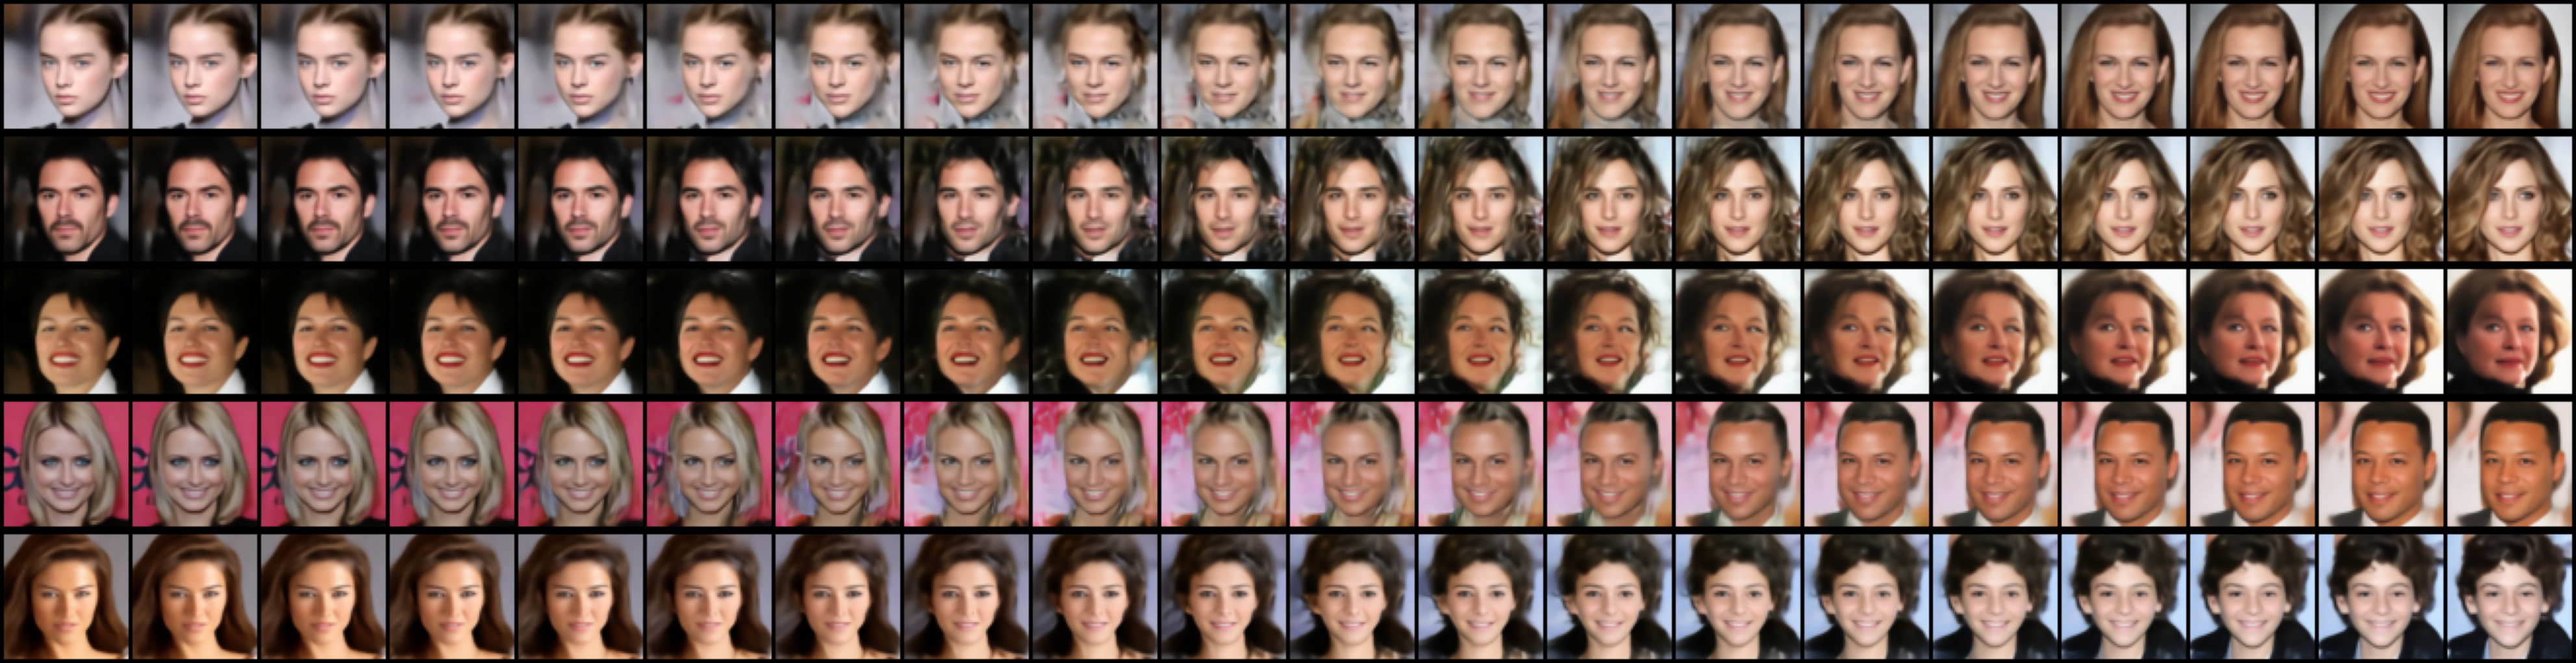
\includegraphics[width=0.7\linewidth]{figures/appendix/interpolation.png}
    \caption{Linear interpolation between the particles learned on the CelebA64 training set.}
    \label{fig:train_intp}
\end{figure}
\subsection{Evolution of the Particle Cloud}
We also visualize how the particle cloud $z_{0}^{1:M, 1:N}$ evolves through the gradient flow. To achieve this, we save the particle cloud at training epochs $\{0,5,10,15,20,25,30,50,75,90\}$ and pass them through the decoder $g_\phi$ (\Cref{fig:evo_cifar,fig:evo_celeba}). We note that there is an intriguing perceptual similarity between the particle evolution and the posterior mean $\mathbb{E}[ x_0 | x_t]$ of a diffusion model. For comparison, we show the evolution of the posterior mean predicted in \Cref{fig:evo_ddim_cifar,fig:evo_ddim_celeba}. The posterior mean is computed by a pretrained score network taken from \citet{song2022denoisingdiffusionimplicitmodels} in the pixel space via Tweedie's formula \citep{efron2011tweedie}: $\mathbb{E}[ x_0| x_t] \approx  (\sqrt{\bar{\alpha}_t})^{-1} [  x_t + \sigma_t^2 \nabla_{ x_t} \vs_\theta( x_t, t)]$, where $\sigma_t^2$ is the variance of the reverse process and $\vs_\theta( x_t, t)$ is the score estimating network.
We remark that there have been several recent works attempting to delineate the connection between diffusion and gradient flow \citep{yiMonoFlowRethinkingDivergence2023,huangGANsGradientFlows2023,franceschiUnifyingGANsScorebased2023}. Our method can be thought as an attempt of learning the gradient flow via a diffusion model.
\begin{figure}[htbp] 
    \centering
    \begin{subfigure}{0.35\linewidth}
         \centering
         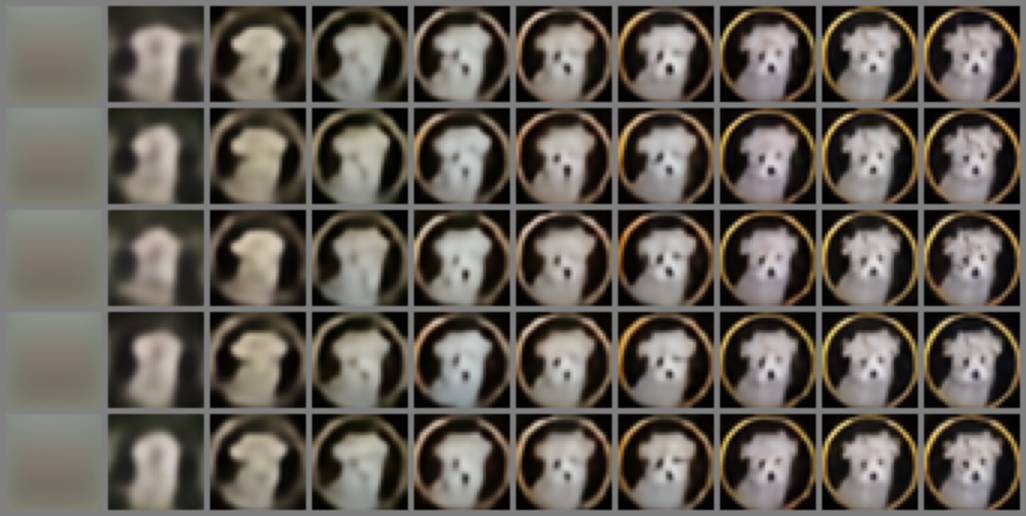
\includegraphics[width=\linewidth]{figures/appendix/evolution_cifar_14650.png}
         \caption{CIFAR-10}
         \label{fig:evo_cifar}
    \end{subfigure}
    \hspace{0.2cm}
    \begin{subfigure}{0.35\linewidth}
         \centering
         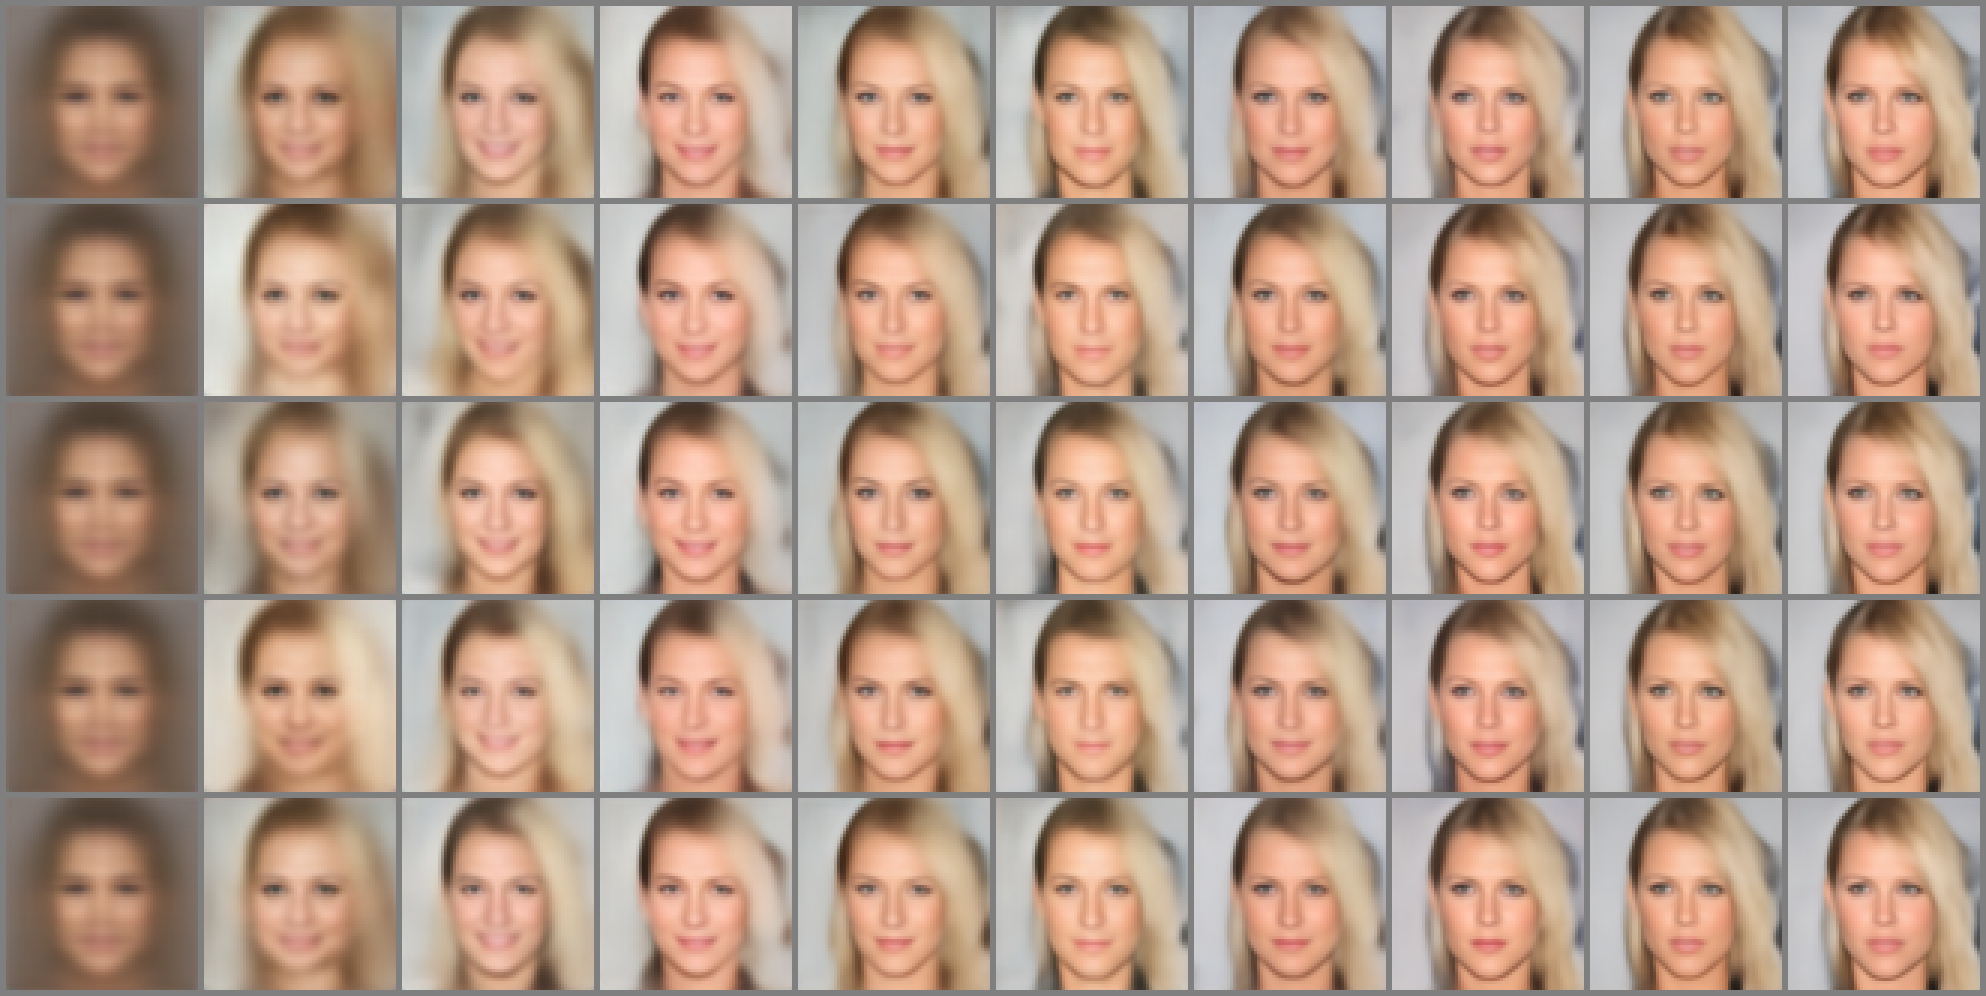
\includegraphics[width=\linewidth]{figures/appendix/evolution_celeba_14986.png}
         \caption{CelebA64}
         \label{fig:evo_celeba}
    \end{subfigure}
    \caption{Evolution of the particle cloud of \gls*{IPLD} trained on the CIFAR-10 and CelebA64 dataset with $5$ particles. Zoom in to view the details better.}
\end{figure}
\begin{figure}[htbp]
    \centering
    \begin{subfigure}{0.35\linewidth}
         \centering
         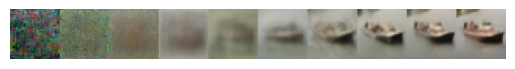
\includegraphics[width=\linewidth]{figures/appendix/ddim_cifar.png}
         \caption{CIFAR-10}
         \label{fig:evo_ddim_cifar}
    \end{subfigure}
    \hspace{0.2cm}
    \begin{subfigure}{0.35\linewidth}
         \centering
         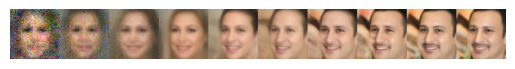
\includegraphics[width=\linewidth]{figures/appendix/ddim_celeba.png}
         \caption{CelebA64}
         \label{fig:evo_ddim_celeba}
    \end{subfigure}
    \caption{Evolution of the predicted $\mathbb{E}[x_0| x_t]$ of \gls*{DDPM} trained on the CIFAR-10 and CelebA64 dataset.}
\end{figure}

\subsection{Ablation on Diffusion Weighting}
As reported in \citet{hodenoisingdiffusionprobabilistic2020,kingmaunderstandingdiffusionobjectives2023}, using the simplified diffusion objective can yield samples with better visual quality. To verify this effect within our framework, we compare two variants of our model: \gls*{IPLD} likelihood using the diffusion loss in \eqref{app_eq:diffusion_likelihood} and \gls*{IPLD} usual using the loss in \eqref{eq_app:simplified_diffusion}. We train all models with the same training hyperparameters specified in \Cref{app:image_exp_details}.
\begin{table}[htp]
    \centering
    \begin{tabular}{lcc}
\hline
& SVHN           & CIFAR-10        \\ \hline
\gls*{IPLD} usual & 17.55     &  51.60     \\
\gls*{IPLD} likelihood & 18.62 & 53.22  \\
\hline
\end{tabular}
    \vspace{0.2cm}
    \caption{Ablation study on diffusion weighting.  The final \gls*{FID} scores are reported.}
    \label{tab:app_ablate_likelihood}
\end{table}
The results in Table \ref{tab:app_ablate_likelihood} show that the simplified objective yields a consistently better FID score, which aligns with prior findings.

\subsection{Ablation on Two Stage Training}
\label{app:2stage_ablate}
\citet{leng2025repaeunlockingvaeendtoend} hypothesized that backpropogating the diffusion loss to the \gls*{VAE} directly make the latent space simpler. They suggested this could inadvertently "hack" the denoising objective, leading the diffusion model to simply predict noise from the \gls*{VAE}'s Gaussian approximate posterior.

To investigate this, we conduct an ablation study comparing end-to-end training and two-stage training. We train both models with $1$ particle using the same training hyperparameters; for two-stage training we detach the gradients on the particles before passing them to the diffusion model, hence preventing backpropogating the diffusion loss. We show in \Cref{tab:app_ablate_2stage} that end-to-end training in \gls*{IPLD} does not suffer from the same issue observed in \citet{leng2025repaeunlockingvaeendtoend}. This aligns with the results in \citet{vahdatscorebasedgenerativemodeling2021}, who also found benefits to end-to-end training. It is important to note, however, that both our experiments and those of \citet{vahdatscorebasedgenerativemodeling2021} were conducted on relatively lower-resolution datasets. Therefore, the conclusions drawn here may not directly extrapolate to the larger-scale experimental settings used in \citet{leng2025repaeunlockingvaeendtoend}.
\begin{table}[htp]
    \centering
    \begin{tabular}{lccc}
\hline
& SVHN           & CIFAR-10      & CelebA64    \\ \hline
\gls*{IPLD} usual & 17.55     &  51.60    & 22.86   \\
\gls*{IPLD} detached & 19.07 & 52.96 &  23.19 \\
\hline
\end{tabular}
    \vspace{0.2cm}
    \caption{Ablation study on two-stage training.  The final \gls*{FID} scores are reported.}
    \label{tab:app_ablate_2stage}
\end{table}

\subsection{Runtime and Memory Comparisons}
\label{app:runtime-compare}
In \Cref{tab:single_gpu_performance}, we benchmark the peak memory usage and walltime for a single forward-backward pass with a batch size of 64 on a single A6000 GPU (48GB) for both \gls*{DiffusionVAE} and \gls*{IPLD}:
\begin{table}[h!]
\centering
\caption{Performance comparison on a single A6000 GPU. Lower values are better.}
\label{tab:single_gpu_performance}
\begin{tabular}{
  l
  S[table-format=2.2]
  S[table-format=1.2]
}
\toprule
\textbf{Method} & {\textbf{Peak Memory (GB) $\downarrow$}} & {\textbf{Walltime (s) $\downarrow$}} \\
\midrule
\gls*{DiffusionVAE} 1-particle  & 5.19  & 0.15 \\
\gls*{DiffusionVAE} 5-particle  & 17.51 & 0.54 \\
\gls*{DiffusionVAE} 10-particle & 33.89 & 1.01 \\
\midrule
\gls*{IPLD} 1-particle          & 4.19  & 0.12 \\
\gls*{IPLD} 5-particle          & 17.26 & 0.49 \\
\gls*{IPLD} 10-particle         & 33.62 & 0.98 \\
\bottomrule
\end{tabular}
\end{table}
Using \texttt{torchrec} \citep{torchrec} and custom sharding strategies enabled by it, we implement a distributed version of \gls*{IPLD} by allocating each accelerator a different subset of the particles (cf. \Cref{sec:pratical-alg}). The results in \Cref{tab:distributed_gpu_performance} confirms the scalability of our algorithm.
\begin{table}[h!]
\centering
\caption{Performance of our custom distributed \gls*{IPLD} implementation on two A6000 GPUs. Lower values are better.}
\label{tab:distributed_gpu_performance}
\begin{tabular}{
  l
  S[table-format=2.2]
  S[table-format=1.2]
}
\toprule
\textbf{Method} & {\textbf{Peak Memory (GB) $\downarrow$}} & {\textbf{Walltime (s) $\downarrow$}} \\
\midrule
\gls*{IPLD} 1-particle  & 2.81  & 0.09 \\
\gls*{IPLD} 5-particle  & 9.62  & 0.29 \\
\gls*{IPLD} 10-particle & 17.95 & 0.56 \\
\bottomrule
\end{tabular}
\end{table}

\subsection{Additional Uncurated Samples}
\label{app:additional_samples}
We present additional uncurated samples of \gls*{IPLD} trained with 10 particles on CIFAR-10, SVHN, and CelebA64 dataset produced by the DDIM sampler \citep{song2022denoisingdiffusionimplicitmodels} with 100 NFEs. We remark that only the CelebA64 samples in the main text have been curated for better visualization. 


\begin{figure}[htbp]
    \centering
    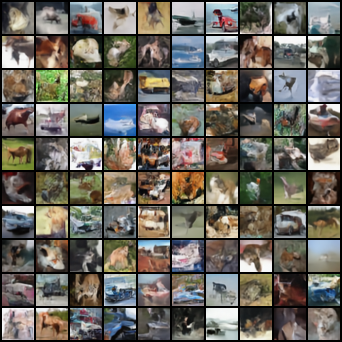
\includegraphics[width=0.5\linewidth]{figures/appendix/cifar_uncurated.png}
    \caption{Uncurated samples on CIFAR-10.}
\end{figure}

\begin{figure}[htbp]
    \centering
    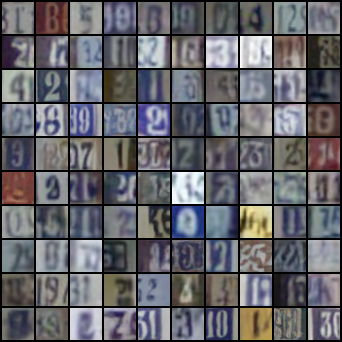
\includegraphics[width=0.5\linewidth]{figures/appendix/svhn_uncurated.png}
    \caption{Uncurated samples on SVHN.}
\end{figure}
\begin{figure}[htbp]
    \centering
    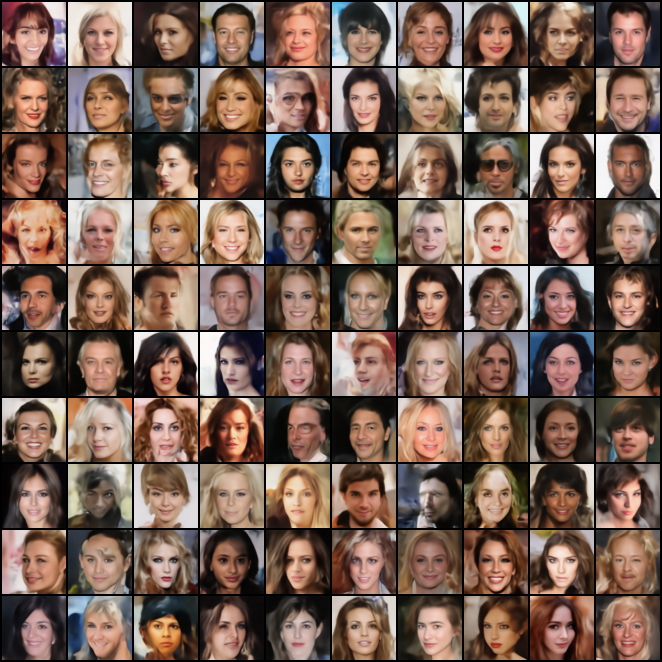
\includegraphics[width=0.5\linewidth]{figures/appendix/celeba64_uncurated.png}
    \caption{Uncurated samples on CelebA64.}
\end{figure}



